\documentclass[12pt,twoside]{book}
\usepackage[margin=1.2in]{geometry}
\usepackage[toc,page]{appendix}
\usepackage{graphicx}
\usepackage[square,numbers]{natbib}
\usepackage{lipsum}
\usepackage{caption}
\usepackage{pdfpages}
\usepackage{url}
\usepackage{MnSymbol,wasysym}
\usepackage{xcolor}
\usepackage{booktabs} % Per linee orizzontali professionali (\toprule, etc.)
\usepackage{graphicx} % Per il comando \resizebox
\usepackage{amsmath}  % Per simboli matematici
\usepackage{float}
\usepackage{rotating}
\usepackage{booktabs}     % per \toprule, \midrule, \bottomrule
\usepackage{array}

\begin{document}

%\captionsetup[figure]{margin=1.5cm,font=small,labelfont={bf},name={Figure},labelsep=colon,textfont={it}}
%\captionsetup[table]{margin=1.5cm,font=small,labelfont={bf},name={Table},labelsep=colon,textfont={it}}
%\SetLipsumDefault{1}

\frontmatter

\begin{titlepage}

% -------------------------------------------------------------------
% You need to edit the details here
% -------------------------------------------------------------------

\begin{center}
{\LARGE University of Bari Aldo Moro}\\[0.25cm]
{\Large Department of Computer Science}\\[1cm]
%{\large \emph{A thesis submitted in partial fulfillment of the requirements for the\\degree of Doctor of Philosophy in Computer Science}}\\[2.5cm]
\linespread{1.2}\huge {\bfseries One-For-All: Un prober per riconoscerli tutti}\\[1.5cm]
\linespread{1}
\includegraphics[width=3.5cm]{images/uniba-logo.png}\\[1.5cm]
{\Large\bf Emanuele Fontana}\\[1cm]
%\large \emph{Supervisor:}\\
%Dr.~Gennaro Vessio\\[1cm] 
\vspace{\fill}
\today
\end{center}

\end{titlepage}

% -------------------------------------------------------------------
% Declaration
% -------------------------------------------------------------------

%\newpage
%\section*{\Large Declaration}

%All sentences or passages quoted in this document from other people's work have been specifically acknowledged by clear cross-referencing to author, work and page(s). Any illustrations that are not the work of the author of this report have been used with the explicit permission of the originator and are specifically acknowledged.  I understand that failure to do this amounts to plagiarism and will be considered grounds for failure.\\[1cm]

%\noindent Name:\\[1mm]
%\rule[1em]{25em}{0.5pt}

%\noindent Signature:\\[1mm]
%\rule[1em]{25em}{0.5pt}

%\noindent Date:\\[1mm]
%\rule[1em]{25em}{0.5pt}

% \includepdf[pages=-]{forms/form.pdf}

%\chapter*{\Large \center Acknowledgement}

Do not forget to acknowledge the supervisor \smiley{}

\textcolor{orange}{PLEASE, FOLLOW THE GUIDELINES GIVEN IN THIS TEMPLATE IN EACH CHAPTER, ESPECIALLY IN CHAPTER 2!}

% -------------------------------------------------------------------
% Abstract
% -------------------------------------------------------------------

\chapter*{\Large \center Abstract}

I Large Language Models hanno dimostrato capacità eccezionali in numerosi compiti di elaborazione del linguaggio naturale, ma soffrono ancora del problema critico delle "allucinazioni", ovvero la generazione di informazioni fattualmente errate presentate con elevata confidenza. Sebbene l'analisi degli stati interni dei modelli (probing) si sia rivelata efficace per rilevare queste anomalie, la maggior parte degli approcci attuali richiede l'addestramento di classificatori specifici per ogni singola architettura, limitandone la scalabilità e l'applicabilità generale.

Questo lavoro esplora la fattibilità di un "prober universale" per il rilevamento delle allucinazioni, indagando se e come le capacità di rilevamento apprese su un modello "Trainer" possano essere trasferite a un modello "Tester" diverso. Abbiamo sviluppato e confrontato diverse metodologie di allineamento degli spazi latenti, spaziando da approcci ibridi e proiezioni non lineari. 

I risultati dimostrano che il trasferimento delle feature legate alla veridicità è altamente efficace, specialmente quando si utilizza l'approccio \textit{One-For-All}. È emerso che l'allineamento degli spazi latenti appreso in contesti più semplici \textcolor{red}{n che senso semplice?} \textcolor{blue}{ho aspresso meglio il concetto ora} è sorprendentemente robusto e trasferibile anche a contesti più complessi, permettendo di mantenere elevate prestazioni di rilevamento. Al contrario, l'allineamento appreso su dati complessi e rumorosi mostra una minore capacità di generalizzazione verso compiti più semplici.

Questo lavoro evidenzia il potenziale delle tecniche di allineamento per la creazione di sistemi di sicurezza cross-model, delineando al contempo i limiti attuali della trasferibilità delle rappresentazioni interne per compiti di ragionamento avanzato.

% -------------------------------------------------------------------
% Contents, list of figures, list of tables
% -------------------------------------------------------------------

\tableofcontents
\listoffigures
\listoftables

% -------------------------------------------------------------------
% Main sections (as required)
% -------------------------------------------------------------------

\mainmatter

\chapter{Introduzione}



\section{Scopi e Obiettivi}
Il rilascio di GPT-3 \cite{GPT3} aperto al pubblico da parte di OpenAI ha segnato una svolta significativa nel Natural Language Processing (NLP), aprendo la strada a una nuova era di modelli di linguaggio di grandi dimensioni (LLM) in grado poter mantenere una conversazione in maniera fluida e naturale come una persona. Il rilascio del ChatBot è stato solo l'inizio: ora gli LLM sono utilizzati in una vasta gamma di applicazioni e sono ormai uno strumento irrinunciabili sia in ambito privato che accademico che industriale, il loro utilizzo è pressocchè sconfinato.

Tuttavia, uno dei principali ostacoli all'adozione diffusa e sicura di queste tecnologie in ambiti critici è il fenomeno delle
 \textit{allucinazioni}. Nonostante la coerenza sintattica, gli LLM tendono occasionalmente a generare informazioni fattualmente errate o inventate con un alto grado di confidenza. In contesti come l'assistenza sanitaria, il supporto legale o l'educazione, tali allucinazioni possono portare a conseguenze gravi (es. diagnosi errate, consigli legali sbagliati o diffusione di disinformazione). Questo comportamento deriva dalla natura stocastica degli LLM: questi ultimi non sanno contare o effettuare un ragionamento logico basato su regole e fatti: la loro abilità nel produrre il testo dipende esclusivamente dalle statistiche apprese durante la fase di addestramento su grandi corpora testuali. Si parla di \textit{next token prediction}: un LLM dunque, dato il contesto (cioè l'insieme dei token precedenti), predice il token successivo più probabile in base alle distribuzioni apprese (possiamo pensare a un token come a una parola o parte di essa).
Un esempio classico di allucinazione presente nei primissimi LLM è:
\begin{quote}
    \textbf{Utente:} How many r's are there in the word strawberries?\\
    \textbf{LLM:} 2
\end{quote}

Attualmente, le tecniche per mitigare questo problema si basano spesso sulla verifica fattuale esterna (\textit{retrieval-augmented generation}), sul \textit{fine-tuning} specifico o sulle \textit{Chain of Thought} (CoT), ma queste tecniche non sono infallibili ed è dunque cruciale capire quando un modello sta allucinando e quando no.

Il \textit{probing} delle attivazioni interne (o \textit{probing classifiers}) rappresenta una soluzione innovativa a questo problema. Questa metodologia consente di analizzare lo stato interno del modello durante la generazione, ipotizzando che l'informazione sulla veridicità di un'affermazione sia codificata nello spazio latente dei neuroni, indipendentemente dall'output testuale finale il quale viene generato stocasticamente in quanto influenzato da molteplici fattori (temperature, top-k sampling, ecc.). 
Diversi studi recenti hanno dimostrato che è possibile addestrare classificatori lineari semplici per distinguere le affermazioni vere da quelle false osservando le attivazioni dei layer interni e che in genere le attivazioni relative alle allucinazioni e quelle relative alle risposte corrette tendono a essere facilmente separabili \cite{Geometry}

Tuttavia, la maggior parte delle ricerche si è concentrata sulla creazione di probe specifici per un singolo modello o una specifica architettura, lasciando relativamente inesplorato il problema della trasferibilità.
Questo lavoro si propone di studiare se esiste una rappresentazione universale delle allucinazioni nei LLM, indipendentemente dall'architettura sottostante. In particolare, si mira a sviluppare un \textit{prober} generale capace di rilevare le allucinazioni in diversi modelli senza la necessità di un addestramento specifico per ciascuno di essi (al più con un allineamento preliminare tra gli spazi latenti, essendo questi ultimi diversi tra modelli differenti).

Gli obiettivi principali di questa progetto sono:
\begin{itemize}
    \item Analizzare e confrontare le attivazioni interne di diverse famiglie di LLM (es. Qwen, Falcon) per identificare pattern comuni associati al fenomeno dell'allucinazione.
    \item Sviluppare e valutare metodologie di allineamento (lineari e non lineari) tra gli spazi latenti di un modello \textit{trainer} e un modello \textit{tester}.
    \item Costruire un \textit{prober} universale capace di trasferire la capacità di rilevamento delle allucinazioni da un modello all'altro senza supervisione aggiuntiva sul modello target.
\end{itemize}


\section{Panoramica del documento}

Il resto del progetto è strutturato come seguee:
\begin{itemize}
    \item \textbf{Capitolo 2: Background} - Backroung teorico e panoramica delle tecniche esistenti per il rilevamento delle allucinazioni nei LLM.
    \item \textbf{Capitolo 3: Metodologia} - Descrizione dettagliata delle architetture utilizzate, delle tecniche di allineamento e del design del prober universale.
    \item \textbf{Capitolo 4: Risultati} - Presentazione dei risultati ottenuti
    \item \textbf{Capitolo 5:Discussione} - Discussione dei risultati ottenuti
    \item \textbf{Capitolo 6: Studi Cross-Domain}: Utilizzo cross-domain del prober One-For-All
    \item \textbf{Capitolo 7: Conclusioni} : Conclusioni finali e proposta lavori futuri
\end{itemize}

\chapter{Background}

In questo capitolo verranno introdotti i concetti di base necessari per comprendere il lavoro svolto. Verranno dunque presentati il concetto di Deep Learning, il concetto dell'attenzione, i Large Language Models (LLM), il fenomeno delle allucinazioni e il probing.


\section{Deep Learning}
Negli ultimi anni il \textit{Deep Learning} ha rivoluzionato il campo dell'intelligenza artificiale, permettendo di raggiungere risultati straordinari in molteplici ambiti, tra cui il riconoscimento delle immagini, l'elaborazione del linguaggio naturale e i giochi. Il Deep Learning non è altro che una brance del Machine Learning (a sua volta branca dell'Intelligenza Artificiale) ed è basato sull'utilizzo di reti neurali profonde (Deep Neural Networks, DNN) per apprendere rappresentazioni complesse dei dati. La sostanziale differenza tra il Deep Learning e il Machine Learning tradizionale è nella rappresentazione dei dati da fornire all'algoritmo: nel Machine Learning tradizionale (DecisionTrees, SVM, etc.) è necessario fornire delle feature ingegnerizzate a mano, mentre nel Deep Learning le reti neurali sono in grado di apprendere automaticamente le rappresentazioni più utili per il compito da svolgere direttamente dai dati grezzi.
\begin{figure}[H]
    \centering
    \includegraphics[width=0.6\textwidth]{images/AI.png}
    \caption{Rappresentazione delle branche dell'Intelligenza Artificiale}
    \label{fig:Artificial Intelligence}
\end{figure}

\subsection{Cenni storici}
Molti pensano che il Deep Learning sia una tecnologia estremamente recente, fantascienza fino a prima di ChatGPT. in realtà le basi teoriche del Deep Learning risalgono agli anni '40 con i primi modelli come il Perceptron di Rosenblatt. Tuttavia a causa limitazioni computazionali, teoriche (Vanishing Gradient Problem) e di disponibilità dei dati, il Deep Learning non ha potuto esprimere tutto il suo potenziale fino agli anni 2000. Con l'avvento delle Graphics Processing Units (GPU), nate per il rendering grafico e il gaming, è stato possibile accelerare notevolmente i calcoli necessari per l'addestramento delle reti neurali profonde. Le GPU, a differenza delle CPU, sono progettate per eseguire un set limitato di operazioni semplici in parallelo, rendendole ideali per le operazioni matriciali e vettoriali tipiche del Deep Learning. Inoltre, la disponibilità di grandi dataset, come ImageNet, ha permesso alle reti neurali di apprendere rappresentazioni più robuste e generalizzabili. Infine, i progressi teorici, come l'introduzione di nuove funzioni di attivazione (ReLU), tecniche di regolarizzazione (Dropout) e algoritmi di ottimizzazione (Adam), hanno ulteriormente migliorato le prestazioni delle reti neurali profonde.
\begin{figure}[H]
    \centering
    \includegraphics[width=0.8\textwidth]{images/DLTimeline.png}
    \caption{Timeline dei principali eventi storici nel campo del Deep Learning}
    \label{fig:Deep Learning Timeline}
    
\end{figure}
\
\subsection{Architettura e addestramento delle DNN}
Le reti neurali profonde sono costituite da molti strati (layer) di neuroni artificiali collegati tra loro (come fossero neuroni di un cervello biologico). Il primo layer è l'input layer, che riceve i dati grezzi, mentre l'ultimo layer è l'output layer, che produce le predizioni finali: la configurazione dell'output layer dipende dal tipo di compito da svolgere (classificazione, regressione, etc.). Tra l'input e l'output layer ci sono diversi hidden layer, che trasformano progressivamente i dati attraverso operazioni lineari (pesi e bias) e non lineari (funzioni di attivazione come ReLU, Sigmoid, Tanh). L'addestramento delle DNN avviene in 2 fasi principali:
\begin{itemize}
    \item \textbf{Forward propagation}: i dati di input vengono propagati attraverso la rete, calcolando le attivazioni di ogni neurone fino a produrre l'output finale. Questo output viene confrontato con il valore target (ground truth) utilizzando una funzione di perdita (loss function) che misura l'errore della predizione. I dati scorrono dunque dall'input layer all'output layer.
    \item \textbf{Backward propagation}: utilizzando l'algoritmo di backpropagation, l'errore calcolato viene propagato all'indietro attraverso la rete. Utilizzando la regola della catena, si calcolano i gradienti rispetto alla loss function e questi vengono propagati all'indietro per aggiornare i pesi e i bias della rete utilizzando un algoritmo di ottimizzazione (come Stochastic Gradient Descent, Adam, etc.). I dati scorrono dunque dall'output layer all'input layer.
\end{itemize}

\begin{figure}
    \centering
    \includegraphics[width=0.8\textwidth]{images/BackProp.png}
    \caption{Rappresentazione della forward e backward propagation in una rete neurale}
    \label{fig:Neural Network Forward Backward}
\end{figure}
\section{Panoramica sui Transformer}
Il meccannismo della self-attention è stato introdotto per la prima volta nel 2017 da Vaswani et al. nel paper "Attention is All You Need" \textcolor{red}{TODO:cita} ed è alla base dell'architettura Transformer, i quali hanno rivoluzionato il campo dell'elaborazione del linguaggio naturale (NLP) e non solo, grazie alla loro capacità di catturare relazioni a lungo raggio nei dati sequenziali in modo più efficiente rispetto ai modelli precedenti come RNN e loro varianti. La differenza cruciale tra i transformer e i modelli precendenti risiede nell'elaborazione dell'input: le RNN elaborato i dati in modo sequenziale, mantenendo uno stato nascosto che cattura le informazioni precedenti, mentre i transformer utilizzano il meccanismo di self-attention per elaborare l'intera sequenza contemporaneamente, permettendo di catturare relazioni tra parole indipendentemente dalla loro distanza nella sequenza. Con un input motlo lungo le RNN tendono a dimenticare le informazioni iniziali mentre i transformer non hanno questo problema. 
\subsection{Architettura dei Transformer}
\begin{figure}[H]
    \centering
    \includegraphics[width=0.8\textwidth]{images/Transformer.png}
    \caption{Architettura di un Transformer}
    \label{fig:Transformer Architecture}
\end{figure}
Un transformer è composto da due blocchi principali: \textit{Encoder} e \textit{Decoder}.
\subsubsection{Encoder}
L'encoder è costituito da una serie di strati identici posti in sequenza, ciascuno dei quali contiene:
\begin{itemize}
    \item \textbf{Multi-Head Self-Attention}: questo meccanismo consente al modello di focalizzarsi su diverse parti della sequenza di input contemporaneamente, catturando relazioni complesse tra le parole.
    \item \textbf{Layer Normalization e Residual Connections}: per migliorare la stabilità dell'addestramento e facilitare il flusso del gradiente, ogni sottostrato è seguito da una normalizzazione e da una connessione residua.
    \item \textbf{Feed-Forward Neural Network (FFNN)}: ogni strato dell'encoder contiene una rete neurale feed-forward completamente connessa che elabora ulteriormente le rappresentazioni ottenute dalla self-attention.
    \item Un altro strato di Layer Normalization e Residual Connections.
\end{itemize}
Il ruolo principale dell'encoder è quello di trasformare la sequenza di input in una rappresentazione interna (embedding) che cattura le relazioni semantiche tra le parole.

\subsubsection{Decoder}
Il decoder è anch'esso costituito da una serie di strati identici posti in sequenza, ciascuno dei quali contiene:
\begin{itemize}
    \item \textbf{Masked Multi-Head Self-Attention}: simile al meccanismo nell'encoder, ma con una maschera che impedisce al modello di "guardare avanti" nella sequenza di output durante l'addestramento, garantendo che la generazione delle parole avvenga in modo autoregressivo.
    \item \textbf{Layer Normalization e Residual Connections}: analogamente all'encoder, per migliorare la stabilità dell'addestramento.
    \item \textbf{Multi-Head Attention sull'Output dell'Encoder}: questo meccanismo consente al decoder di focalizzarsi sulle parti rilevanti della rappresentazione dell'input generata dall'encoder.
    \item Un altro strato di Layer Normalization e Residual Connections.
    \item \textbf{Feed-Forward Neural Network (FFNN)}: come nell'encoder, per elaborare ulteriormente le rappresentazioni.
    \item Un ulteriore strato di Layer Normalization e Residual Connections.
\end{itemize}


\subsection{Meccanismo di Self-Attention}
\begin{figure}[H]
    \centering
    \includegraphics[width=0.6\textwidth]{images/Attn.png}
    \caption{Rappresentazione del meccanismo di Self-Attention}
    \label{fig:Self Attention Mechanism}
\end{figure}
Il meccanismo di self-attention consente al modello di pesare l'importanza delle diverse parole nella sequenza di input quando si elabora una particolare parola. Il calcolo della self-attention avviene attraverso tre matrici distinte: Query (Q), Key (K) e Value (V). La formula per calcolare l'attenzione è la seguente:
\begin{equation}
    \text{Attention}(Q, K, V) = \text{softmax}\left(\frac{QK^T}{\sqrt{d_k}}\right)V
\end{equation}
dove \(d_k\) è la dimensione delle chiavi. La softmax normalizza i punteggi di attenzione, permettendo al modello di concentrarsi sulle parole più rilevanti. Il meccanismo di multi-head attention estende questo concetto eseguendo più calcoli di attenzione in parallelo, permettendo al modello di catturare diverse tipologie relazioni tra le parole.


\section{Large Language Models (LLM)}
I Large Language Models (LLM) rappresentano l'evoluzione naturale delle architetture Transformer applicate su scala massiva. Un LLM è essenzialmente un modello probabilistico addestrato su enormi corpora di testo (nell'ordine di trilioni di token) con l'obiettivo fondamentale di prevedere il token successivo in una sequenza, dato il contesto precedente. Formalmente, data una sequenza di token \( x = (x_1, x_2, ..., x_t) \), il modello cerca di stimare la distribuzione di probabilità condizionata \( P(x_{t+1} | x_1, ..., x_t) \).



L'evoluzione dagli scorsi modelli di NLP agli attuali LLM (come la serie GPT, Llama, e Claude) è caratterizzata dal fenomeno dello \textit{scaling law} \textcolor{red}{TODO: citare Kaplan et al.}, secondo cui le prestazioni del modello migliorano in modo prevedibile all'aumentare del numero di parametri, della quantità di dati di addestramento e della potenza di calcolo.

Il ciclo di vita tipico di un LLM si divide in fasi distinte:
\begin{enumerate}
    \item \textbf{Pre-training}: È la fase più costosa computazionalmente. Il modello viene addestrato in modo auto-supervisionato su vasti dataset (web crawl, libri, codice) per apprendere la struttura del linguaggio, la logica e una vasta gamma di conoscenze generali. L'obiettivo è minimizzare la \textit{Cross-Entropy Loss} tra la distribuzione prevista e il token reale successivo.
    \item \textbf{Supervised Fine-Tuning (SFT)}: Il modello pre-addestrato (detto "Base") viene ulteriormente addestrato su un dataset più piccolo e curato di istruzioni e risposte (formato prompt-response). Questo permette al modello di imparare a seguire le istruzioni dell'utente e di adottare un formato conversazionale.
    \item \textbf{Alignment (RLHF/DPO)}: Per garantire che il modello sia sicuro e allineato con i valori umani, vengono applicate tecniche come il \textit{Reinforcement Learning from Human Feedback} (RLHF) o la \textit{Direct Preference Optimization} (DPO). In questa fase, il modello viene penalizzato se genera contenuti tossici, bias o non utili.
\end{enumerate}

Una caratteristica emergente degli LLM è la capacità di \textit{In-Context Learning}, ovvero la capacità di apprendere nuovi task semplicemente osservando alcuni esempi nel prompt, senza aggiornare i pesi del modello.

\section{Allucinazioni nei LLM}
Nonostante le straordinarie capacità generative, gli LLM soffrono di una limitazione critica nota come ``allucinazione''. Nel contesto dell'intelligenza artificiale, un'allucinazione si verifica quando un modello genera un output che è sintatticamente corretto e fluido, ma fattualmente errato, logicamente incoerente o non fedele alla sorgente di input fornita.



Le allucinazioni possono essere categorizzate principalmente in due tipologie:
\begin{itemize}
    \item \textbf{Allucinazioni di Fattualità (Factuality Hallucinations)}: Il modello genera informazioni che contraddicono la conoscenza del mondo reale. Un esempio tipico è l'attribuzione di una citazione alla persona sbagliata o l'invenzione di eventi storici mai accaduti. Questo fenomeno è spesso legato alla natura probabilistica del modello, che tende a completare pattern linguistici piuttosto che recuperare fatti deterministici.
    \item \textbf{Allucinazioni di Fedeltà (Faithfulness Hallucinations)}: Si verificano in task come la summarization o la Question Answering basata su documenti (RAG), quando il modello genera informazioni che non sono presenti nel testo sorgente o le contraddicono, pur essendo magari vere nel mondo reale (allucinazione estrinseca) o false (allucinazione intrinseca).
\end{itemize}

Le cause delle allucinazioni sono molteplici e includono: la compressione con perdita della conoscenza durante il training, dati di addestramento rumorosi o contraddittori, e la tendenza del modello a privilegiare la fluidità del testo rispetto all'accuratezza fattuale (spesso definita come \textit{sycophancy}, ovvero la tendenza a compiacere l'utente confermando i suoi bias). Rilevare e mitigare le allucinazioni è attualmente una delle sfide più aperte nella ricerca sugli LLM.

\section{Probing}
Il \textit{Probing} (o \textit{Probing Classifiers}) è una tecnica di analisi utilizzata nel campo dell'\textit{Explainable AI} (XAI) per interpretare le rappresentazioni interne delle reti neurali profonde. L'idea fondamentale è che, sebbene gli LLM siano spesso considerati delle ``black box'', le loro attivazioni interne (i valori degli hidden states e degli output dei vari moduli a ogni layer) contengano informazioni ricche e strutturate riguardanti l'input elaborato.



La metodologia standard di probing prevede i seguenti passi:
\begin{enumerate}
    \item \textbf{Estrazione delle attivazioni}: Si fornisce un input al modello (frozen, ovvero con i pesi congelati) e si registrano i vettori di attivazione \( h_l \) generati in uno specifico layer \( l \).
    \item \textbf{Addestramento del Prober}: Si addestra un classificatore supervisionato semplice (spesso una Regressione Lineare o un Perceptron Multistrato semplice) che prende in input le attivazioni \( h_l \) e cerca di predire una specifica proprietà \( y \) dell'input (ad esempio: la parte del discorso, la lunghezza della frase, o, nel caso di questo lavoro, la veridicità dell'affermazione).
    \item \textbf{Valutazione}: Le prestazioni del classificatore indicano quanto l'informazione relativa alla proprietà \( y \) sia codificata linearmente (o non linearmente) in quel particolare layer del modello.
\end{enumerate}

Nel contesto delle allucinazioni, il probing viene utilizzato per investigare se esiste una ``direzione della verità'' nello spazio latente del modello. L'ipotesi è che il modello, internamente, ``sappia'' se sta generando un fatto vero o un'allucinazione, e che questa informazione possa essere decodificata analizzando gli stati interni prima che venga generato l'output testuale finale.

\section{Large Language Models utilizzati}
Per gli esperimenti condotti in questo lavoro, sono stati selezionati due modelli open-weights che rappresentano lo stato dell'arte per le rispettive dimensioni e famiglie architetturali.

\subsection{Qwen2.5-7B}
Qwen2.5-7B è un modello sviluppato da Alibaba Cloud ed è parte della serie Qwen2.5. È un modello \textit{Decoder-only} basato su Transformer con 7 miliardi di parametri. Rispetto ai suoi predecessori, Qwen2.5 introduce diverse ottimizzazioni architetturali:
\begin{itemize}
    \item \textbf{Grouped Query Attention (GQA)}: Utilizza GQA invece della standard Multi-Head Attention per ottimizzare l'uso della memoria della cache KV durante l'inferenza, permettendo contesti più lunghi e una generazione più veloce.
    \item \textbf{SwiGLU Activation}: Sostituisce la classica funzione di attivazione GeLU con SwiGLU, che ha dimostrato empiricamente di migliorare le prestazioni di convergenza.
    \item \textbf{RoPE (Rotary Positional Embeddings)}: Utilizza embeddings posizionali rotativi per gestire meglio le posizioni relative dei token e supportare finestre di contesto molto ampie (fino a 128k token).
\end{itemize}
Il modello è stato pre-addestrato su un corpus massivo e multilingua, dimostrando eccellenti capacità non solo nel ragionamento e nella comprensione del linguaggio, ma anche nel coding e nella matematica, spesso superando modelli di dimensioni simili come Llama-3-8B in vari benchmark.

\subsection{Falcon3-7B-Base}
Falcon3-7B-Base è l'ultima iterazione della famiglia di modelli sviluppati dal Technology Innovation Institute (TII) di Abu Dhabi. Come Qwen, è un modello \textit{causal decoder-only} da 7 miliardi di parametri, ma si distingue per scelte progettuali orientate all'efficienza.
Falcon3 continua la tradizione della serie Falcon concentrandosi sulla qualità dei dati di pre-training (basati sul dataset RefinedWeb, un dataset web rigorosamente filtrato e deduplicato).
A livello architetturale, Falcon3-7B adotta soluzioni moderne per massimizzare il throughput in inferenza. Sebbene le specifiche esatte possano variare tra le versioni (es. l'uso di \textit{Multi-Query Attention} o \textit{FlashAttention}), l'obiettivo principale di Falcon è fornire un modello performante che sia facilmente deployabile su hardware di consumo. Nel contesto di questo lavoro, Falcon3 viene utilizzato come termine di paragone (o modello ``studente'') per verificare la generalizzabilità dei prober addestrati su architetture diverse come Qwen.




\section{Metodologia}

\begin{frame}{Metodologia}
    \framesubtitle{Dataset Utilizzati}
    \begin{itemize}
        \item \textbf{Belief Bank Facts}:
        \begin{itemize}
            \item Fatti affermativi e negati (es. "An eagle is a bird").
            \item 27.416 affermazioni (Bilanciato).
            \item Rilevamento \textit{Factual Hallucinations}.
        \end{itemize}
        \item \textbf{Belief Bank Constraints}:
        \begin{itemize}
            \item Implicazioni e mutue esclusioni.
            \item 25.756 affermazioni.
            \item Rilevamento \textit{Logical Inconsistencies}.
        \end{itemize}
        \item \textbf{HaluEval}:
        \begin{itemize}
            \item Contesti conversazionali complessi.
            \item 10.000 esempi.
        \end{itemize}
    \end{itemize}
\end{frame}



\begin{frame}{Metodologia}
    \textbf{Pipeline di Estrazione}
    \begin{enumerate}
        \item Prompting del modello (es. "Is the fact true?").
        \item Estrazione attivazioni da tutti i layer e componenti (Attention, MLP, Hidden).
        \item Etichettatura basata sulla risposta generata (Yes/No).
    \end{enumerate}

    \textbf{Pipeline generale di addestramento}

    \begin{enumerate}
    \item Addestramento prober sulle attivazioni del modello trainer
    \item Allineamento delle attivazioni in comune tra trainer e tester
    \item Valutazione delle attivazioni allineate del tester sul prober del trainer
    \end{enumerate}
\end{frame}

\begin{frame}{Metodologia: Baseline}
    \framesubtitle{Approccio Lineare}
    \begin{figure}
        \centering
        \includegraphics[width=0.9\textwidth, height=0.7\textheight]{images/modelsss/AppL.png}
        \caption{Pipeline Baseline: Logistic Regression su Trainer, Ridge Regression per allineamento Tester.}
    \end{figure}
\end{frame}

\begin{frame}{Metodologia: Approccio Ibrido}
    \framesubtitle{Allineamento Non-Lineare + Prober Lineare}
    \begin{figure}
        \centering
        \includegraphics[width=0.9\textwidth, height=0.6\textheight]{images/modelsss/AppH.png}
        \caption{Pipeline Ibrida: AlignmentNetwork non-lineare per proiettare il Tester, classificatore lineare fisso.}
    \end{figure}
\end{frame}

\begin{frame}{Metodologia: Approccio Non-Lineare Completo}
    \framesubtitle{Allineamento Non-Lineare + Prober Non-Lineare}
    \begin{figure}
        \centering
        \includegraphics[width=0.9\textwidth, height=0.6\textheight]{images/modelsss/PipeApp1.png}
        \caption{Pipeline Completa: AlignmentNetwork e MLP Prober entrambi non-lineari.}
    \end{figure}
\end{frame}

\begin{frame}{Metodologia: Approccio Non-Lineare Ridotto}
    \framesubtitle{Riduzione Dimensionale con Autoencoder}
    \begin{figure}
        \centering
        \includegraphics[width=0.9\textwidth, height=0.7\textheight]{images/modelsss/PipeApp2.png}
        \caption{Pipeline Ridotta: Autoencoder per ridurre il rumore, poi allineamento nello spazio latente.}
    \end{figure}
\end{frame}

\begin{frame}{Metodologia: One-For-All}
    \framesubtitle{Frozen Head \& Encoder Adaptation}
    \begin{figure}
        \centering
        \includegraphics[width=0.9\textwidth, height=0.7\textheight]{images/modelsss/PipeApp3.png}
        \caption{Pipeline One-For-All: Encoder specifico per modello, Classification Head congelata dal Trainer.}
    \end{figure}
\end{frame}


\section{Risultati}

\begin{frame}{Risultati: Falcon3 e Qwen2.5 su BeliefBankFacts}
    \framesubtitle{Qwen2.5 $\rightarrow$ Falcon3 (Tutti gli approcci)}
    \begin{table}
        \centering
        \resizebox{\textwidth}{!}{
        \begin{tabular}{lllcc}
            \toprule
            \textbf{Trainer $\rightarrow$ Tester} & \textbf{Approach} & \textbf{Type} & \textbf{AUROC (Tr)} & \textbf{AUROC (Te)} \\
            \midrule
            Qwen $\rightarrow$ Falcon & Baseline & attn & 0.999 & 0.992 \\
            Qwen $\rightarrow$ Falcon & HApproach & attn & 0.999 & 0.984 \\
            Qwen $\rightarrow$ Falcon & FullNonLinear & attn & 1.000 & 0.994 \\
            Qwen $\rightarrow$ Falcon & ReducedNonLinear & attn & 0.999 & 0.995 \\
            \textbf{Qwen $\rightarrow$ Falcon} & \textbf{One-For-All} & \textbf{attn} & \textbf{1.000} & \textbf{0.999} \\
            \bottomrule
        \end{tabular}
        }
        \caption{Confronto Approcci (Qwen $\rightarrow$ Falcon)}
        \scriptsize Tr=Trainer, Te=Tester
    \end{table}
    \begin{itemize}
        \item \textbf{One-For-All} e \textbf{FullNonLinear} ottengono i risultati migliori.
        \item \textbf{Baseline} è già molto forte in questo caso.
    \end{itemize}
\end{frame}

\begin{frame}{Risultati: Llama-3.1 e Gemma-2 su BeliefBankFacts}
    \framesubtitle{Gemma-2 $\rightarrow$ Llama-3.1 (Tutti gli approcci)}
    \begin{table}
        \centering
        \resizebox{\textwidth}{!}{
        \begin{tabular}{lllcc}
            \toprule
            \textbf{Trainer $\rightarrow$ Tester} & \textbf{Approach} & \textbf{Type} & \textbf{AUROC (Tr)} & \textbf{AUROC (Te)} \\
            \midrule
            Gemma $\rightarrow$ Llama & Baseline & attn & 0.986 & 0.974 \\
            Gemma $\rightarrow$ Llama & HApproach & attn & 0.986 & 0.961 \\
            Gemma $\rightarrow$ Llama & FullNonLinear & attn & 0.994 & 0.976 \\
            Gemma $\rightarrow$ Llama & ReducedNonLinear & attn & 0.993 & 0.970 \\
            \textbf{Gemma $\rightarrow$ Llama} & \textbf{One-For-All} & \textbf{attn} & \textbf{0.992} & \textbf{0.997} \\
            \bottomrule
        \end{tabular}
        }
        \caption{Confronto Approcci (Gemma $\rightarrow$ Llama)}
        \scriptsize Tr=Trainer, Te=Tester
    \end{table}
    \begin{itemize}
        \item \textbf{One-For-All} mostra un netto miglioramento rispetto alla Baseline.
        \item Gli approcci non lineari (Full/Reduced) non superano One-For-All.
    \end{itemize}
\end{frame}

\begin{frame}{Risultati: Llama-3.1 e Gemma-2 su HaluEval}
    \framesubtitle{Gemma-2 $\rightarrow$ Llama-3.1 (Tutti gli approcci)}
    \begin{table}
        \centering
        \resizebox{\textwidth}{!}{
        \begin{tabular}{lllcc}
            \toprule
            \textbf{Trainer $\rightarrow$ Tester} & \textbf{Approach} & \textbf{Type} & \textbf{AUROC (Tr)} & \textbf{AUROC (Te)} \\
            \midrule
            Gemma $\rightarrow$ Llama & Baseline & attn & 0.767 & 0.853 \\
            Gemma $\rightarrow$ Llama & HApproach & attn & 0.767 & 0.811 \\
            Gemma $\rightarrow$ Llama & FullNonLinear & attn & 0.790 & 0.834 \\
            Gemma $\rightarrow$ Llama & ReducedNonLinear & attn & 0.772 & 0.788 \\
            \textbf{Gemma $\rightarrow$ Llama} & \textbf{One-For-All} & \textbf{attn} & \textbf{0.768} & \textbf{0.855} \\
            \bottomrule
        \end{tabular}
        }
        \caption{Confronto Approcci su HaluEval}
        \scriptsize Tr=Trainer, Te=Tester
    \end{table}
    \begin{itemize}
        \item Su dataset complessi, \textbf{Baseline} rimane molto competitiva.
        \item \textbf{One-For-All} mantiene buone performance ma il gap è ridotto.
    \end{itemize}
\end{frame}

\begin{frame}{Risultati}
    \textbf{Cross-Domain: One-For-All}
    \begin{table}
        \centering
        \resizebox{\textwidth}{!}{
        \begin{tabular}{lllcccccc}
            \toprule
            \textbf{Train Dataset} & \textbf{Test Dataset} & \textbf{Trainer} & \textbf{Tester} & \textbf{Layer} & \textbf{Acc (Tr)} & \textbf{AUROC (Tr)} & \textbf{Acc (Te)} & \textbf{AUROC (Te)} \\
            \midrule
            BBF & HE & Gemma & Llama & attn & 0.985 & 0.993 & 0.995 & 0.997 \\
            BBF & HE & Llama & Gemma & attn & 0.994 & 0.998 & 0.986 & 0.997 \\
            HE & BBF & Gemma & Llama & attn & 0.877 & 0.925 & 0.906 & 0.950 \\
            HE & BBF & Llama & Gemma & attn & 0.907 & 0.948 & 0.885 & 0.932 \\
            \bottomrule
        \end{tabular}
        }
        \caption{Sintesi risultati Cross-Domain (Layer: attn)}
        \scriptsize Tr=Trainer, Te=Tester. Train Dataset = dataset su cui è addestrato l'encoder.
    \end{table}
    \textbf{Osservazione}: L'encoder addestrato su task semplici (BBF) generalizza bene a task complessi (HE), mentre il viceversa funziona peggio.
\end{frame}
\chapter{Discussion}

This chapter discusses the results obtained from the experiments conducted to evaluate the different approaches proposed for hallucination detection in LLMs. The main objective is to analyze the effectiveness of transferring detection capabilities from a "Trainer" model to a "Tester" model through different alignment techniques.

\section{Comparison Between Methods}
The results show that the suggested transferability methods are fairly equivalent to each other, presenting very similar metrics on both the tester and trainer. The study therefore demonstrates that it is possible to transfer probers for hallucination detection between different models, especially for simple factual verification tasks. The \textit{One-For-All} approach proves to be the most promising method for building a "universal prober".

\section{Dataset Analysis}

The results highlight a clear distinction between datasets based on simple facts (BeliefBank) and more complex ones (HaluEval).

\begin{itemize}
    \item \textbf{BeliefBankFacts and BeliefBankCalibration}: On these datasets, all models and approaches achieve very high performance, with accuracies often exceeding 95\%. This suggests that the distinction between true and false statements about general knowledge facts is encoded very clearly and linearly separable in the activation spaces of LLMs. Transferability is therefore high.
    
    \item \textbf{HaluEval}: This dataset proves to be significantly more difficult. Accuracies drop to around 70-80\% for all approaches. In this scenario, the \textit{FullLinear} often clearly outperforms the transfer approaches. This indicates that the "directions" encoding hallucinations in more complex contexts are much more model-specific and less transferable through the tested alignment techniques.
\end{itemize}

\section{Model Analysis}

The comparison between model pairs offers further insights:

\begin{itemize}
    \item \textbf{Falcon3-7B-Base and Qwen2.5-7B}: This pair shows exceptional compatibility on BeliefBankFacts, with nearly perfect transfer results. This could indicate a structural or pre-training similarity that facilitates the alignment of their latent spaces.
    
    \item \textbf{Llama-3.1-8B-Instruct and Gemma-2-9B-IT}: This pair also performs well on BeliefBank, but shows greater difficulties on HaluEval. It is interesting to note that in some cases (e.g., HaluEval), the "tester" outperforms the "trainer", suggesting that some internal representations may be more suitable for hallucination detection in complex contexts.
\end{itemize}

\section{Layer Analysis}

Regarding the layer type (\textit{attn}, \textit{mlp}, \textit{hidden}), no absolute winner emerges across all scenarios. However, it is often noted that \textit{attn} (attention output) and \textit{hidden} (hidden states) activations tend to provide slightly more stable performance compared to \textit{mlp}. The \textit{One-For-All} approach nevertheless demonstrates remarkable robustness regardless of the layer type used, managing to extract useful information from all internal components analyzed.


\chapter{Cross-Domain Studies}
To further evaluate the generalizability of transferred probers, cross-domain experiments were conducted. In this context, the \textit{One-For-All} approach was evaluated by training the alignment on a source dataset ("Train Set") and applying it to project the activations of a target dataset ("Test Set"), while using the Teacher's Head specific to the target dataset. This scenario evaluates the robustness of the learned alignment.

The results, summarized in Table \ref{tab:cross-domain-results}, show that the encoding learned via encoder on simple facts datasets (BeliefBank) transfers with exceptional effectiveness even to the classification head learned on a more complex dataset (HaluEval), allowing the Tester to achieve performance nearly identical to the Trainer (often >99\% accuracy).
Conversely, the encoding learned on HaluEval, while achieving good results, shows a performance drop when transferred to BeliefBank (approximately 87--90\% accuracy), suggesting that the latent space structure learned on complex tasks may be less "universal" or noisier compared to that learned on simple facts.

\begin{table}[H]
\centering
\resizebox{\textwidth}{!}{
\begin{tabular}{lllccccccc}
\toprule
\textbf{Align Train} & \textbf{Target/Head} & \textbf{Teacher} & \textbf{Student} & \textbf{Layer} & \textbf{Acc (Tr)} & \textbf{AUROC (Tr)} & \textbf{Acc (Te)} & \textbf{AUROC (Te)} \\
\midrule
BBC & BBF & Gemma & Llama & attn & 0.991 & 0.999 & 0.995 & 0.999 \\
BBC & BBF & Gemma & Llama & mlp & 0.992 & 0.998 & 0.984 & 0.995 \\
BBC & BBF & Gemma & Llama & hidden & 0.995 & 0.997 & 0.990 & 0.999 \\
BBC & BBF & Llama & Gemma & attn & 0.991 & 0.996 & 0.994 & 0.999 \\
BBC & BBF & Llama & Gemma & mlp & 0.980 & 0.995 & 0.994 & 1.000 \\
BBC & BBF & Llama & Gemma & hidden & 0.993 & 0.999 & 0.993 & 0.999 \\
\midrule
BBC & HE & Gemma & Llama & attn & 0.991 & 0.997 & 0.995 & 0.999 \\
BBC & HE & Gemma & Llama & mlp & 0.993 & 0.997 & 0.984 & 0.993 \\
BBC & HE & Gemma & Llama & hidden & 0.995 & 0.996 & 0.991 & 0.999 \\
BBC & HE & Llama & Gemma & attn & 0.993 & 0.998 & 0.994 & 0.999 \\
BBC & HE & Llama & Gemma & mlp & 0.980 & 0.990 & 0.994 & 1.000 \\
BBC & HE & Llama & Gemma & hidden & 0.993 & 0.998 & 0.993 & 0.999 \\
\midrule
BBF & BBC & Gemma & Llama & attn & 0.986 & 0.997 & 0.994 & 0.997 \\
BBF & BBC & Gemma & Llama & mlp & 0.983 & 0.992 & 0.994 & 0.998 \\
BBF & BBC & Gemma & Llama & hidden & 0.972 & 0.995 & 0.993 & 0.998 \\
BBF & BBC & Llama & Gemma & attn & 0.994 & 0.997 & 0.987 & 0.994 \\
BBF & BBC & Llama & Gemma & mlp & 0.992 & 0.999 & 0.983 & 0.987 \\
BBF & BBC & Llama & Gemma & hidden & 0.992 & 0.999 & 0.977 & 0.986 \\
\midrule
BBF & HE & Gemma & Llama & attn & 0.985 & 0.993 & 0.995 & 0.997 \\
BBF & HE & Gemma & Llama & mlp & 0.984 & 0.989 & 0.994 & 0.998 \\
BBF & HE & Gemma & Llama & hidden & 0.971 & 0.991 & 0.993 & 0.997 \\
BBF & HE & Llama & Gemma & attn & 0.994 & 0.998 & 0.986 & 0.997 \\
BBF & HE & Llama & Gemma & mlp & 0.992 & 1.000 & 0.983 & 0.996 \\
BBF & HE & Llama & Gemma & hidden & 0.991 & 0.996 & 0.979 & 0.996 \\
\midrule
HE & BBC & Gemma & Llama & attn & 0.872 & 0.916 & 0.907 & 0.924 \\
HE & BBC & Gemma & Llama & mlp & 0.873 & 0.928 & 0.905 & 0.950 \\
HE & BBC & Gemma & Llama & hidden & 0.871 & 0.926 & 0.904 & 0.907 \\
HE & BBC & Llama & Gemma & attn & 0.909 & 0.941 & 0.884 & 0.894 \\
HE & BBC & Llama & Gemma & mlp & 0.900 & 0.944 & 0.871 & 0.897 \\
HE & BBC & Llama & Gemma & hidden & 0.893 & 0.935 & 0.880 & 0.928 \\
\midrule
HE & BBF & Gemma & Llama & attn & 0.877 & 0.925 & 0.906 & 0.950 \\
HE & BBF & Gemma & Llama & mlp & 0.872 & 0.924 & 0.903 & 0.945 \\
HE & BBF & Gemma & Llama & hidden & 0.872 & 0.928 & 0.905 & 0.940 \\
HE & BBF & Llama & Gemma & attn & 0.907 & 0.948 & 0.885 & 0.932 \\
HE & BBF & Llama & Gemma & mlp & 0.901 & 0.950 & 0.871 & 0.928 \\
HE & BBF & Llama & Gemma & hidden & 0.897 & 0.935 & 0.880 & 0.929 \\
\bottomrule
\end{tabular}
}
\caption{Cross-Domain Results (One-For-All). Tr=Trainer, Te=Tester, BBC=BeliefBankConstraints, BBF=BeliefBankFacts, HE=HaluEval}
\label{tab:cross-domain-results}
\end{table}



\chapter{Conclusioni}

In questoo capitolo vengono riassunti i principali risultati ottenuti dal lavoro svolto e le prospettive future.

\section{Sintesi dei Risultati}
\textcolor{red}{TODO: Aggiungere una sintesi dei risultati principali ottenuti dagli esperimenti

\section{Lavori Futuri}
Il lavoro svolto può essere proseguito in diverse direzioni:
\begin{itemize}
    \item \textbf{Espansione degli esperimenti}: Ripetere gli esperimenti con diversi modelli e diversi dataset
    \item \textbf{Verifica cross-dataset}: Testare la capacità di generalizzazione del prober su dataset diversi da quelli utilizzati per l'addestramento.
    \item \textbf{Ottimizzazione delle architetture}: Capire quali sono i migliori layer da utilizzare per l'estrazione delle attivazioni e sperimentare
    \item \textbf{Esperimenti multimodali}: Estendere l'approccio a modelli multimodali che integrano testo e immagini.
\end{itemize}
% -------------------------------------------------------------------
% Bibliography
% -------------------------------------------------------------------

\bibliographystyle{plainnat}
\bibliography{main} 

% -------------------------------------------------------------------
% Appendices
% -------------------------------------------------------------------

\begin{appendices}
\chapter{Visualizzazioni PCA}
\label{app:pca_plots}

In questa appendice sono riportate le visualizzazioni complete dell'Analisi delle Componenti Principali (PCA) a 2 dimensioni per tutte le tipologie di layer (Attention, MLP, Hidden) e per entrambi i modelli analizzati (Qwen2.5-7B e Falcon3-7B-Base). I punti rossi rappresentano le istanze allucinate, mentre i punti blu rappresentano le istanze corrette.

\section{Qwen2.5-7B}

\begin{figure}[h]
    \centering
    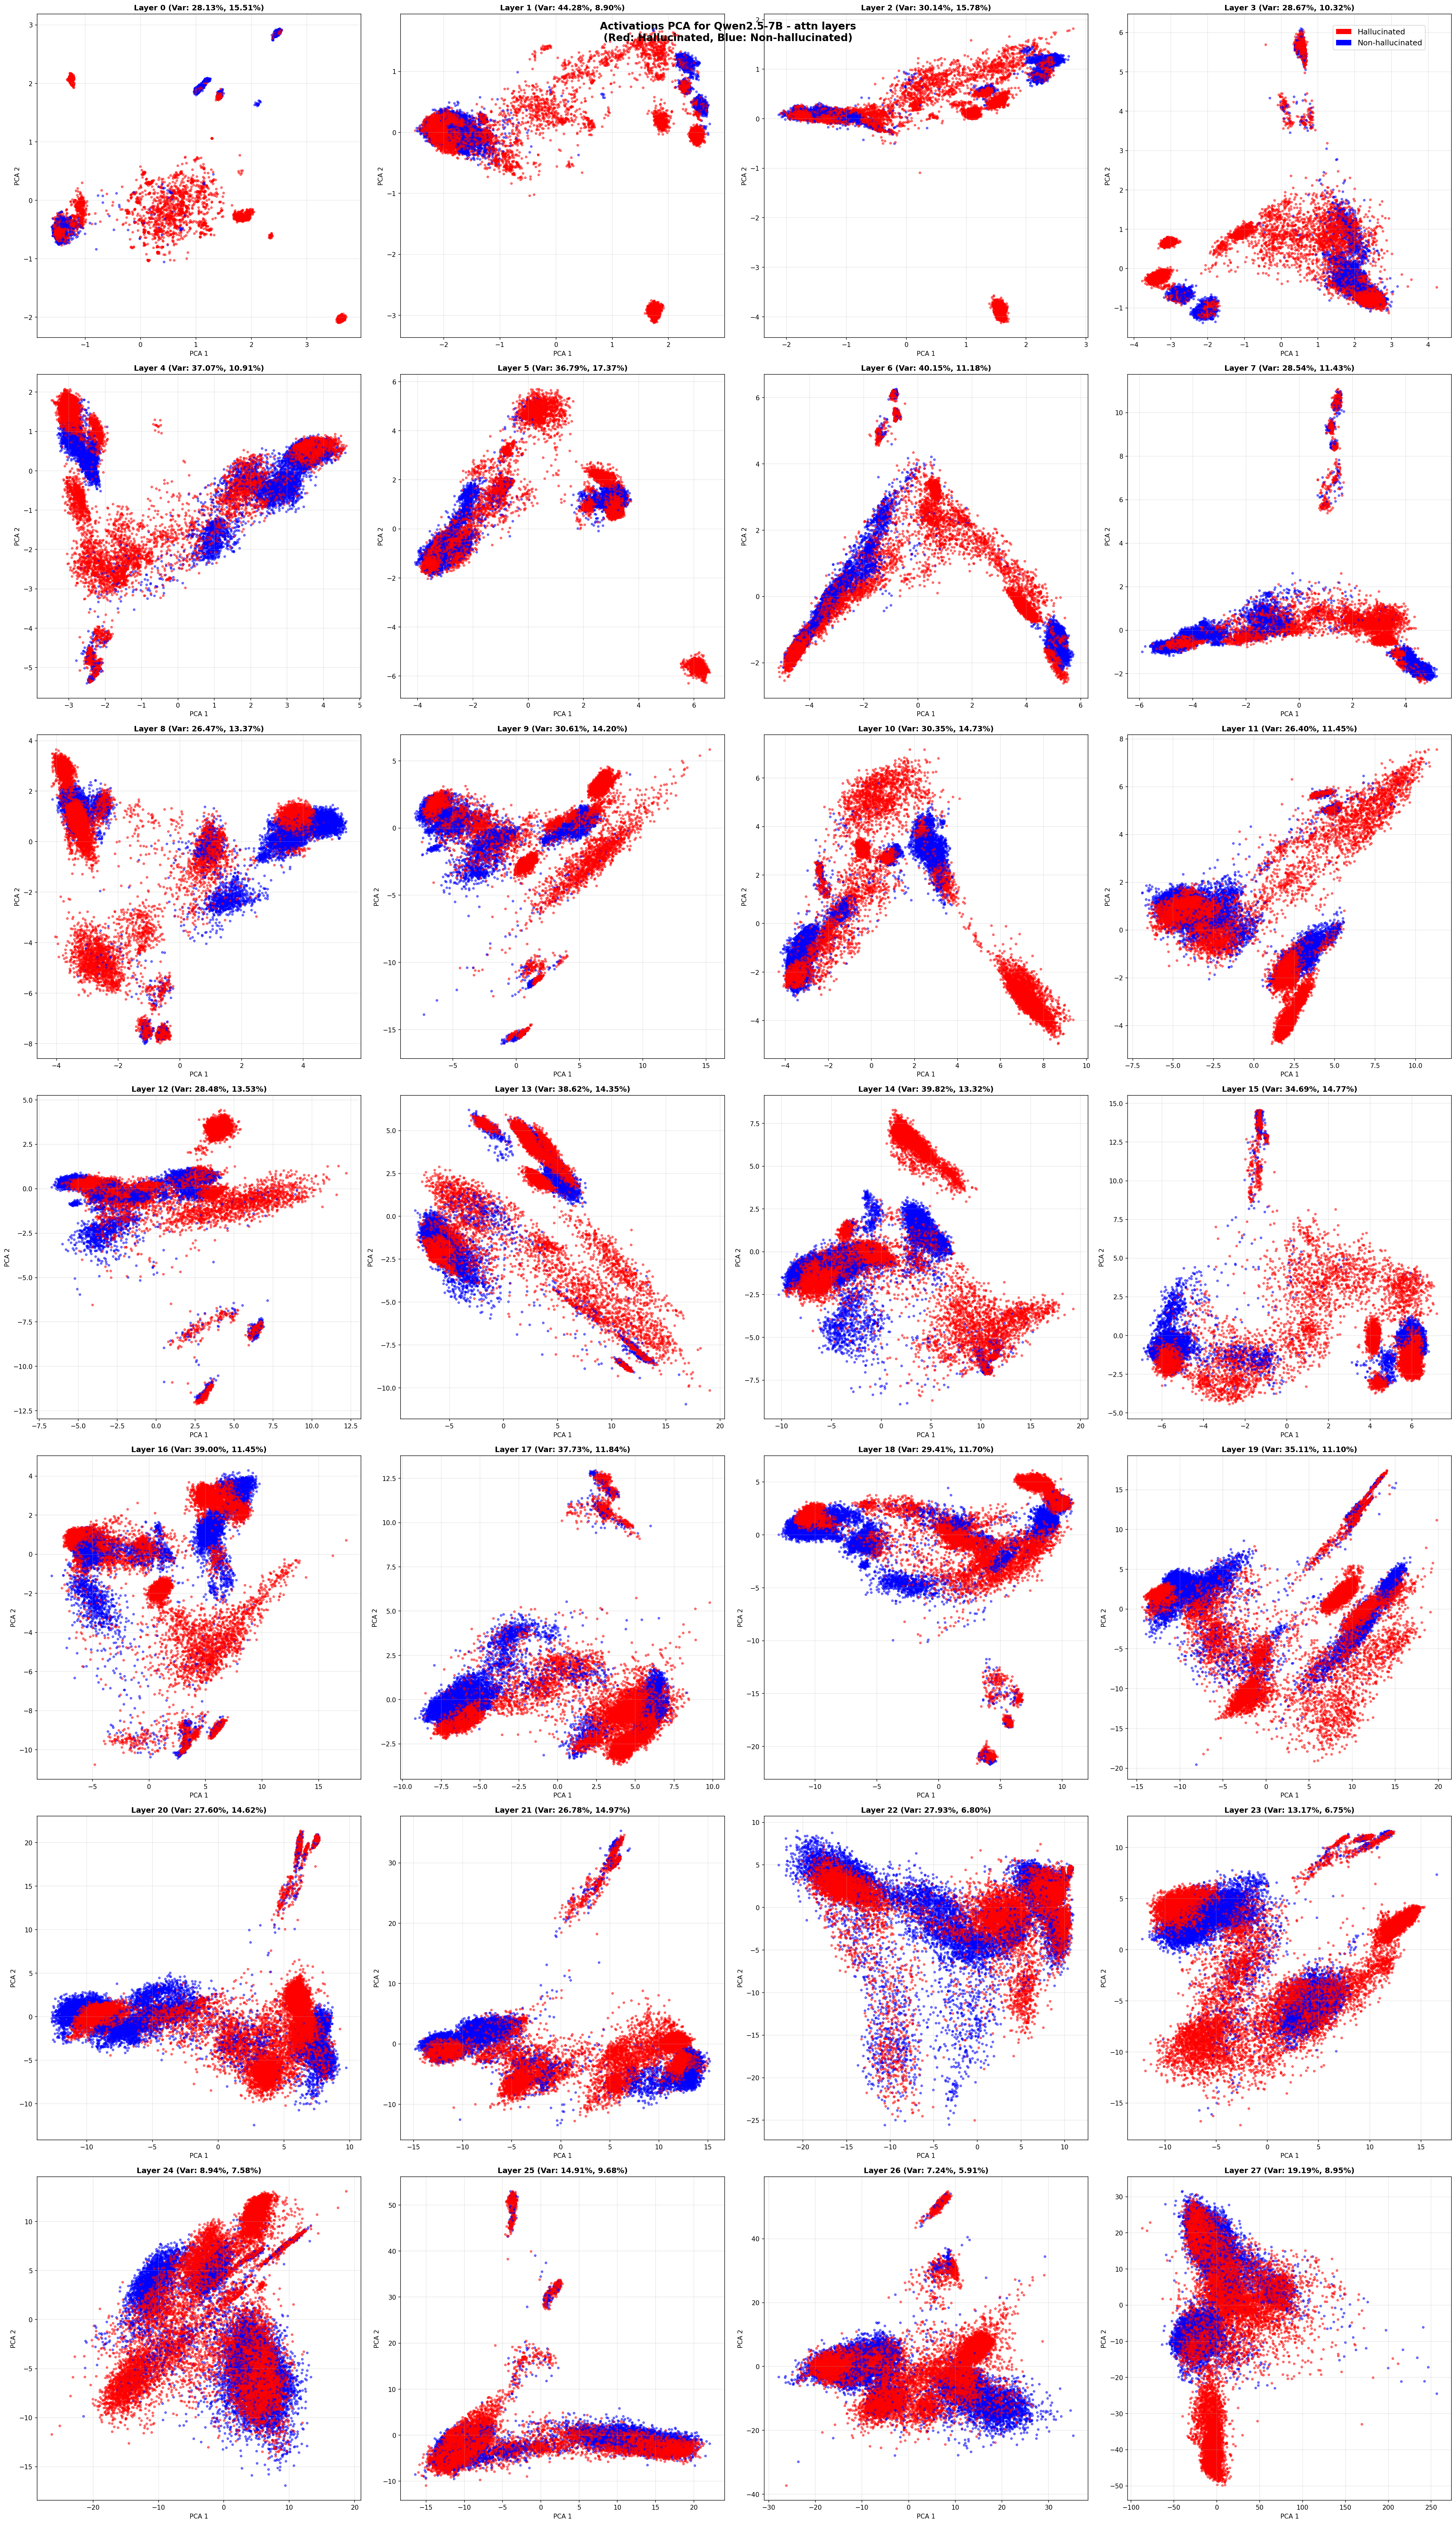
\includegraphics[width=0.9\textwidth]{images/plots/Qwen2.5-7B_belief_bank_attn_activations_PCA.png}
    \caption{PCA 2D - Qwen2.5-7B - Attention Layers}
    \label{fig:pca_qwen_attn}
\end{figure}

\begin{figure}[h]
    \centering
    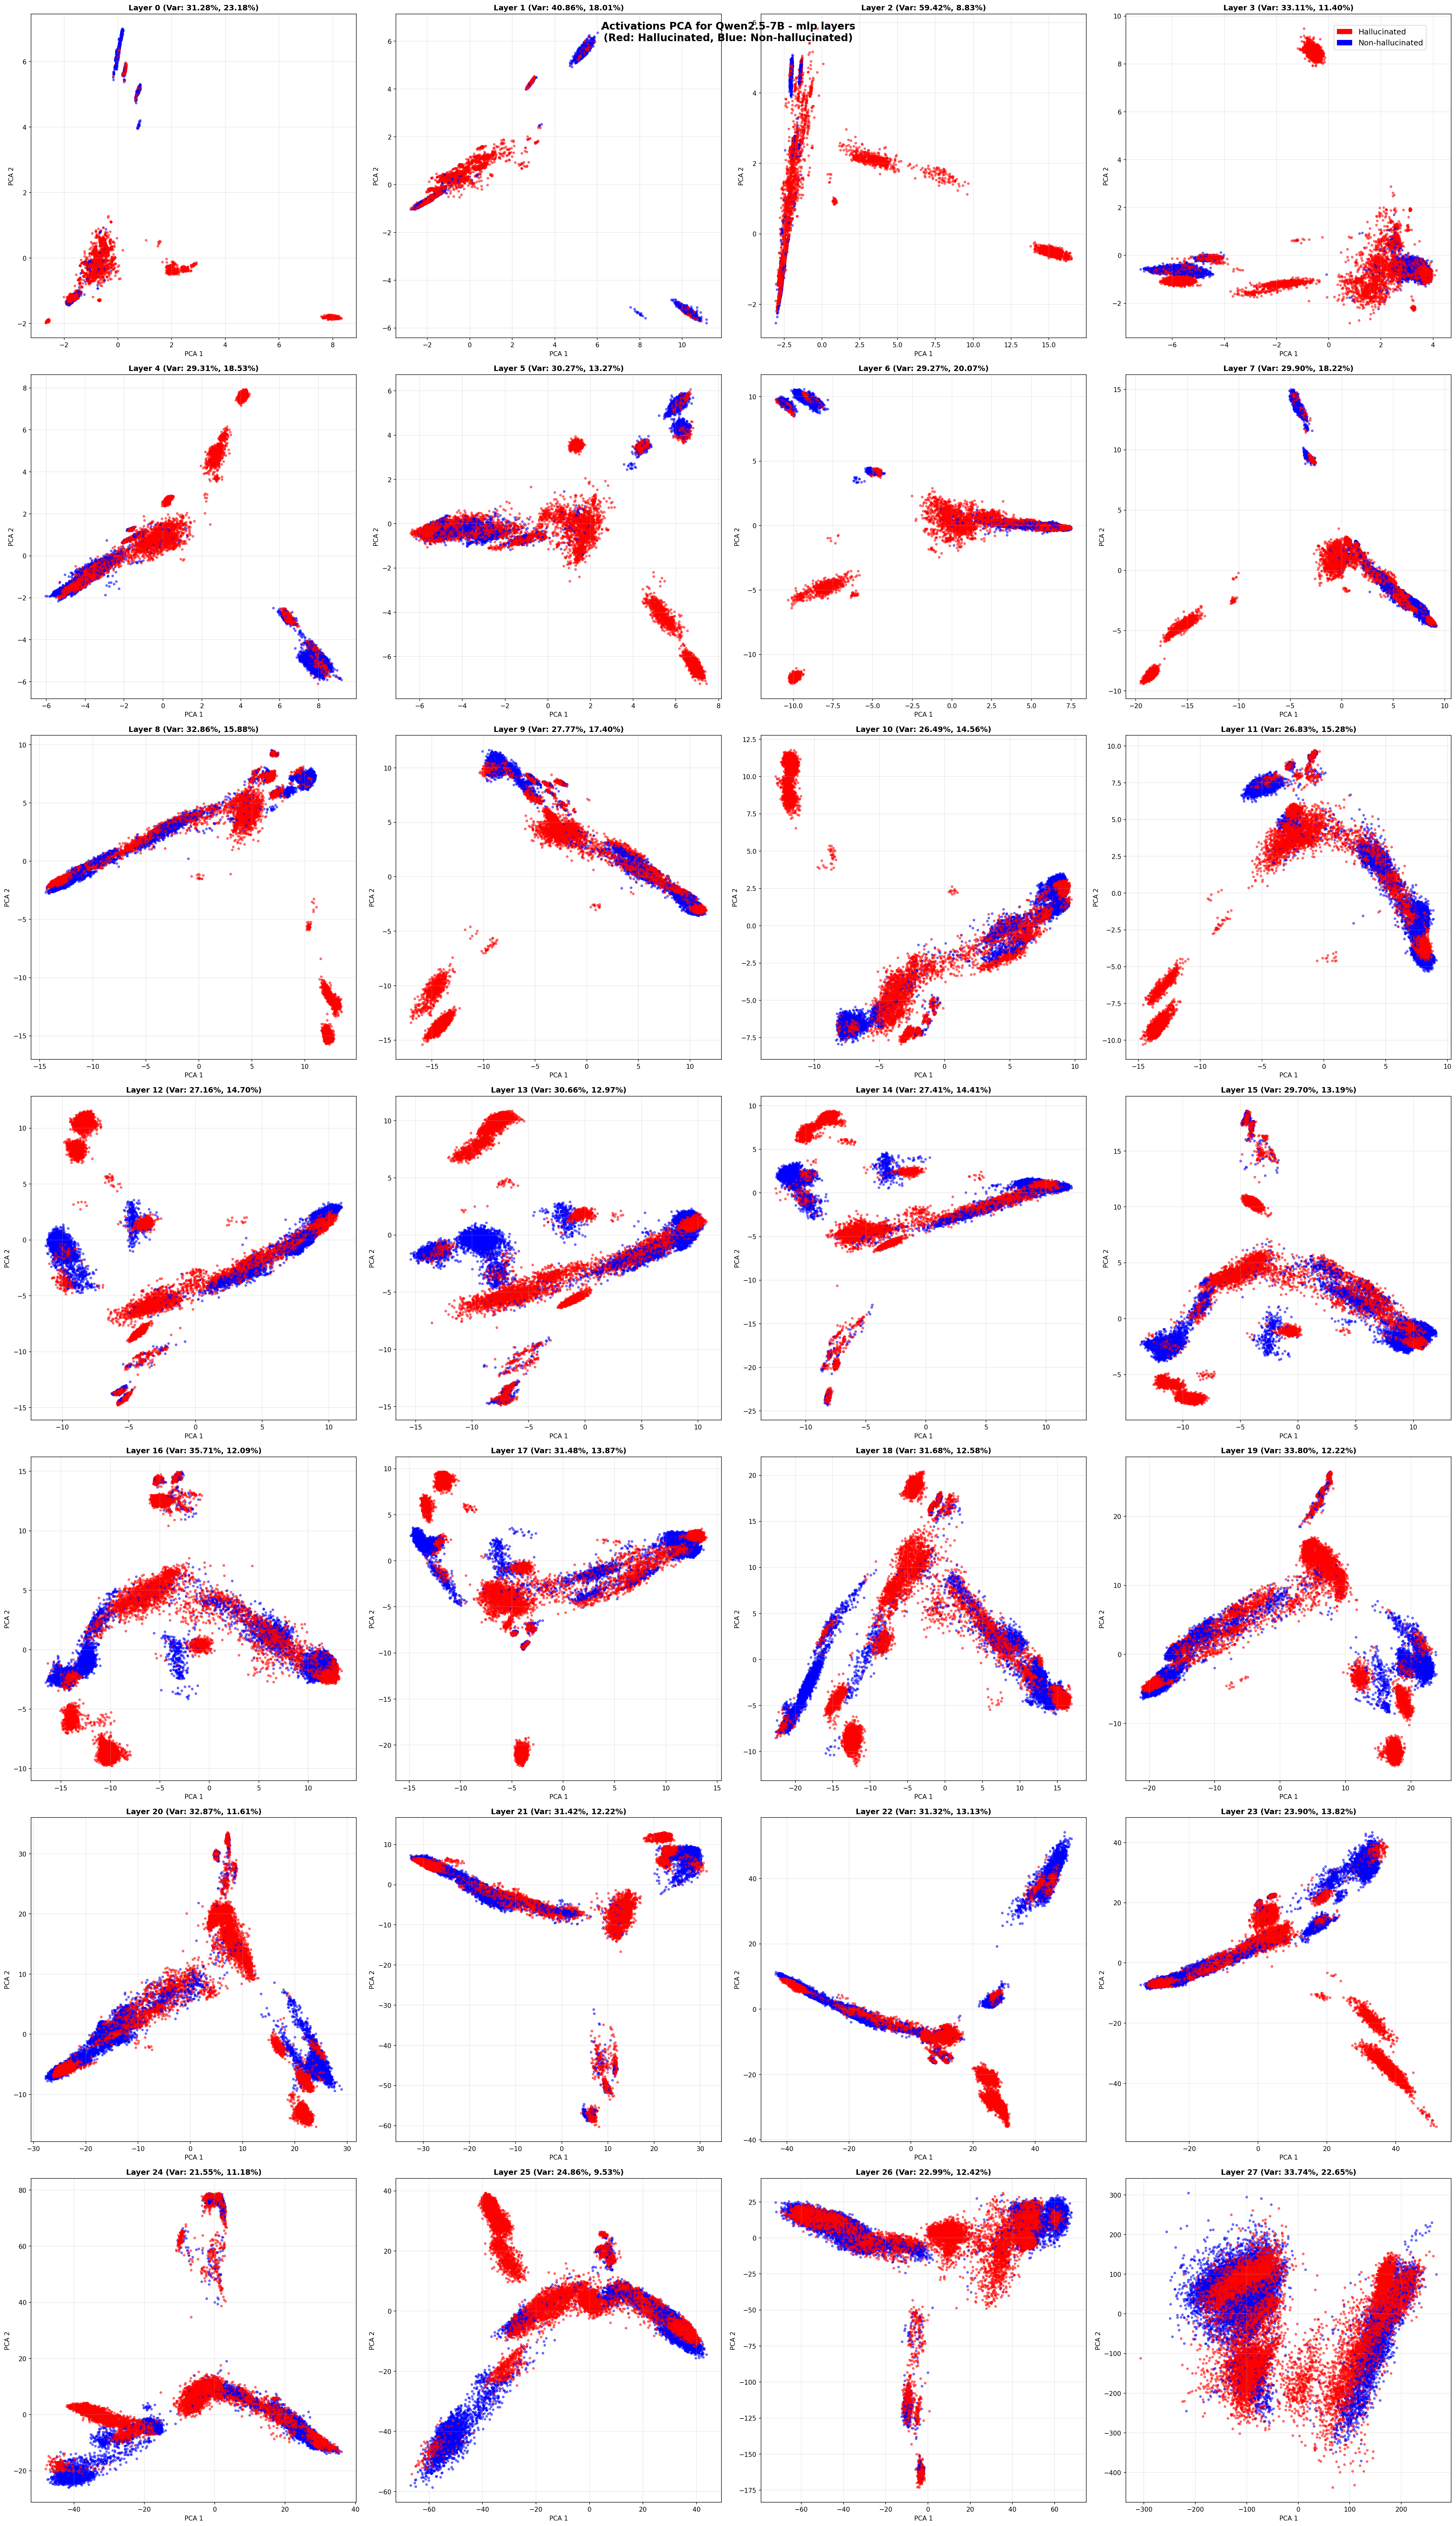
\includegraphics[width=0.9\textwidth]{images/plots/Qwen2.5-7B_belief_bank_mlp_activations_PCA.png}
    \caption{PCA 2D - Qwen2.5-7B - MLP Layers}
    \label{fig:pca_qwen_mlp}
\end{figure}

\begin{figure}[h]
    \centering
    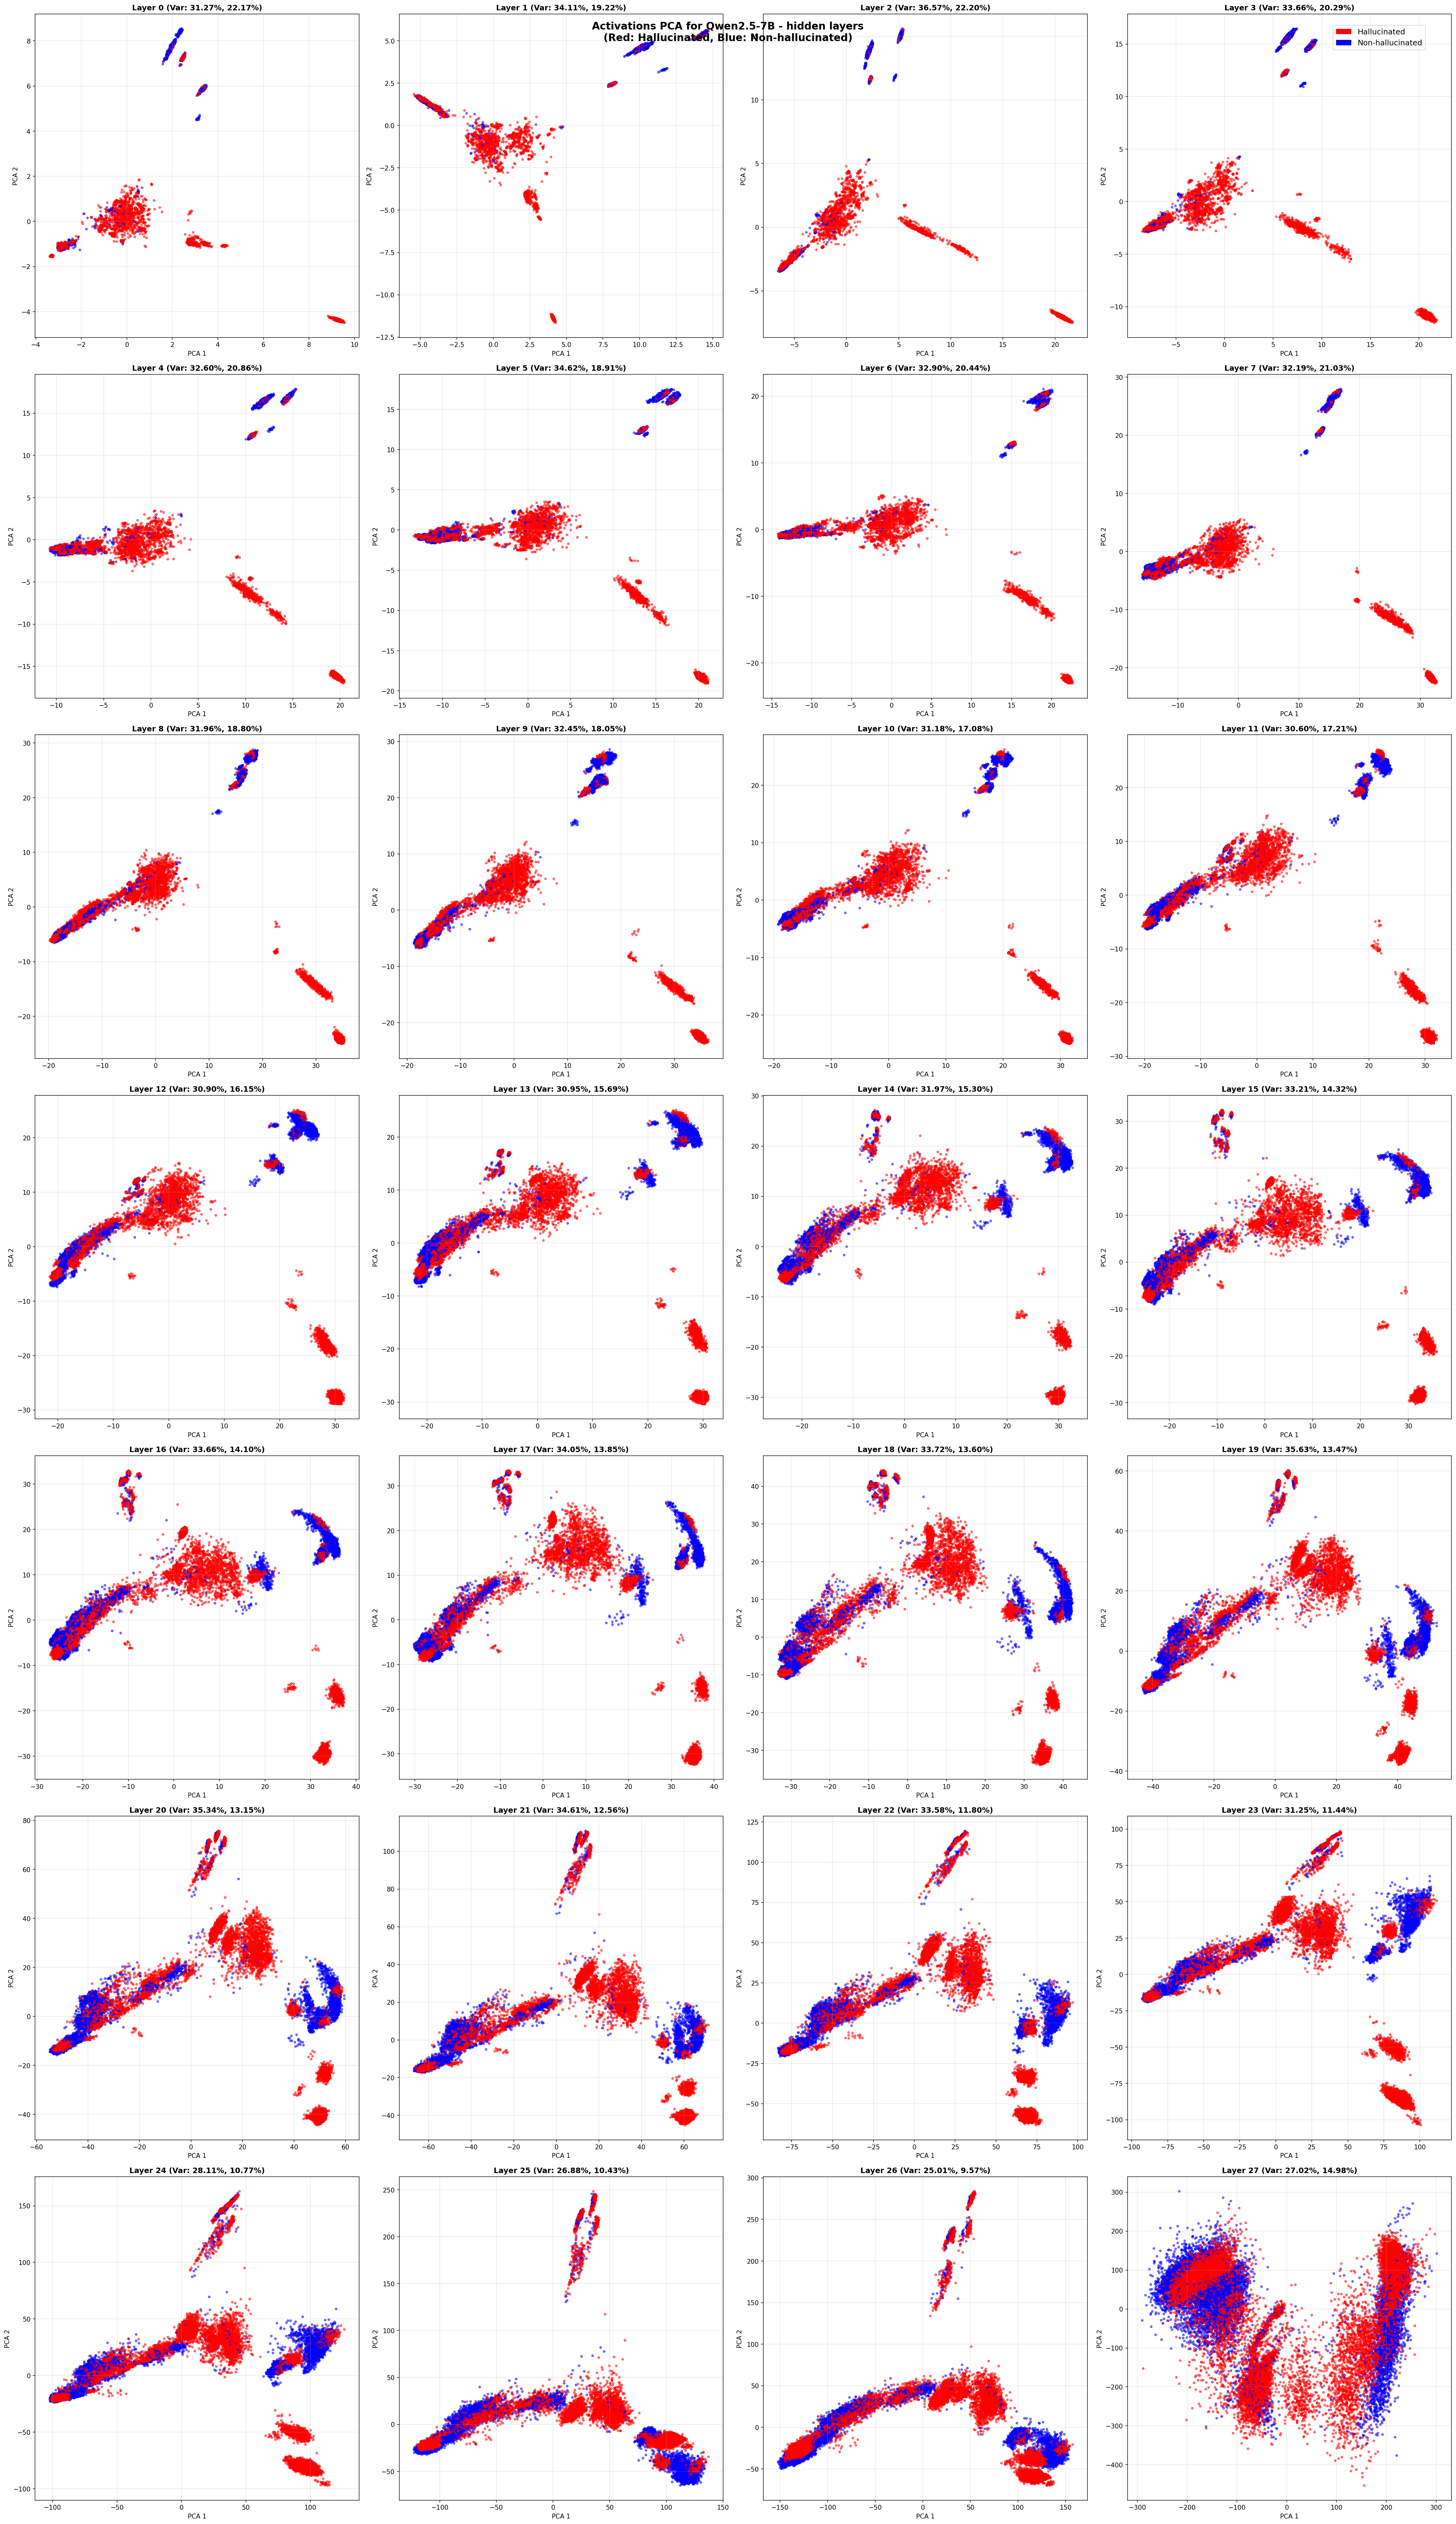
\includegraphics[width=0.9\textwidth]{images/plots/Qwen2.5-7B_belief_bank_hidden_activations_PCA.png}
    \caption{PCA 2D - Qwen2.5-7B - Hidden Layers}
    \label{fig:pca_qwen_hidden}
\end{figure}

\clearpage

\section{Falcon3-7B-Base}

\begin{figure}[h]
    \centering
    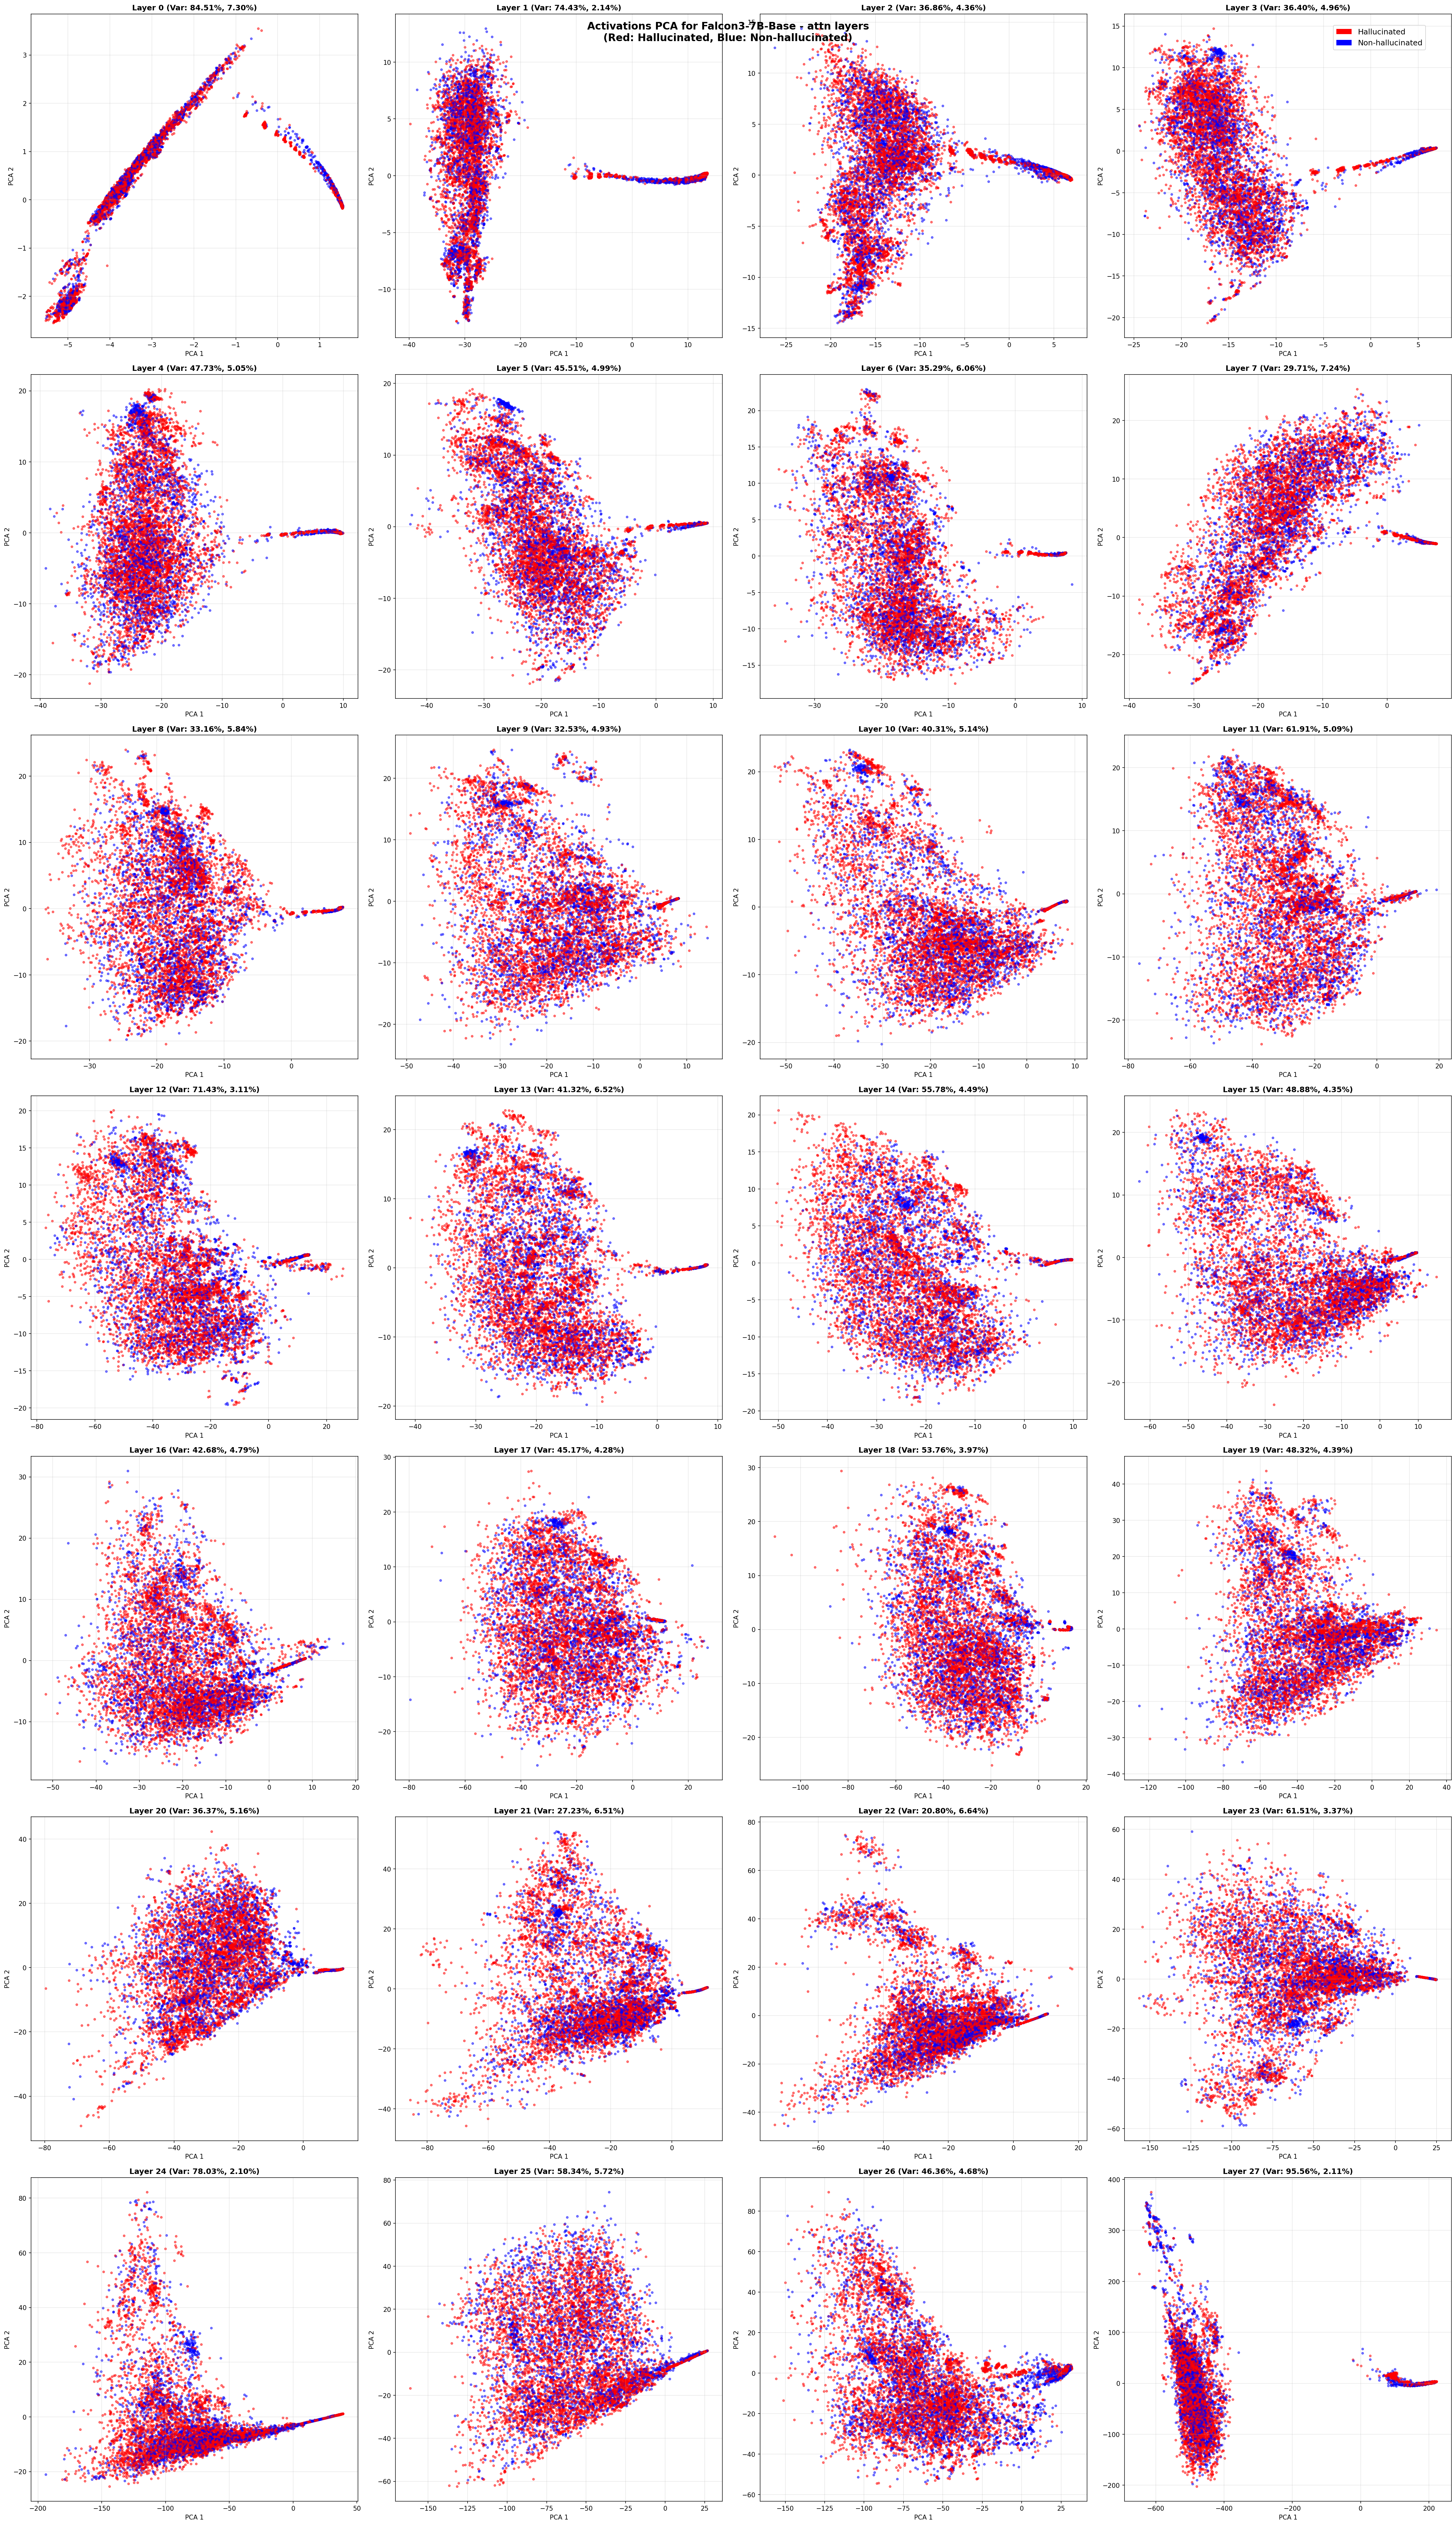
\includegraphics[width=0.9\textwidth]{images/plots/Falcon3-7B-Base_belief_bank_attn_activations_PCA.png}
    \caption{PCA 2D - Falcon3-7B-Base - Attention Layers}
    \label{fig:pca_falcon_attn}
\end{figure}

\begin{figure}[h]
    \centering
    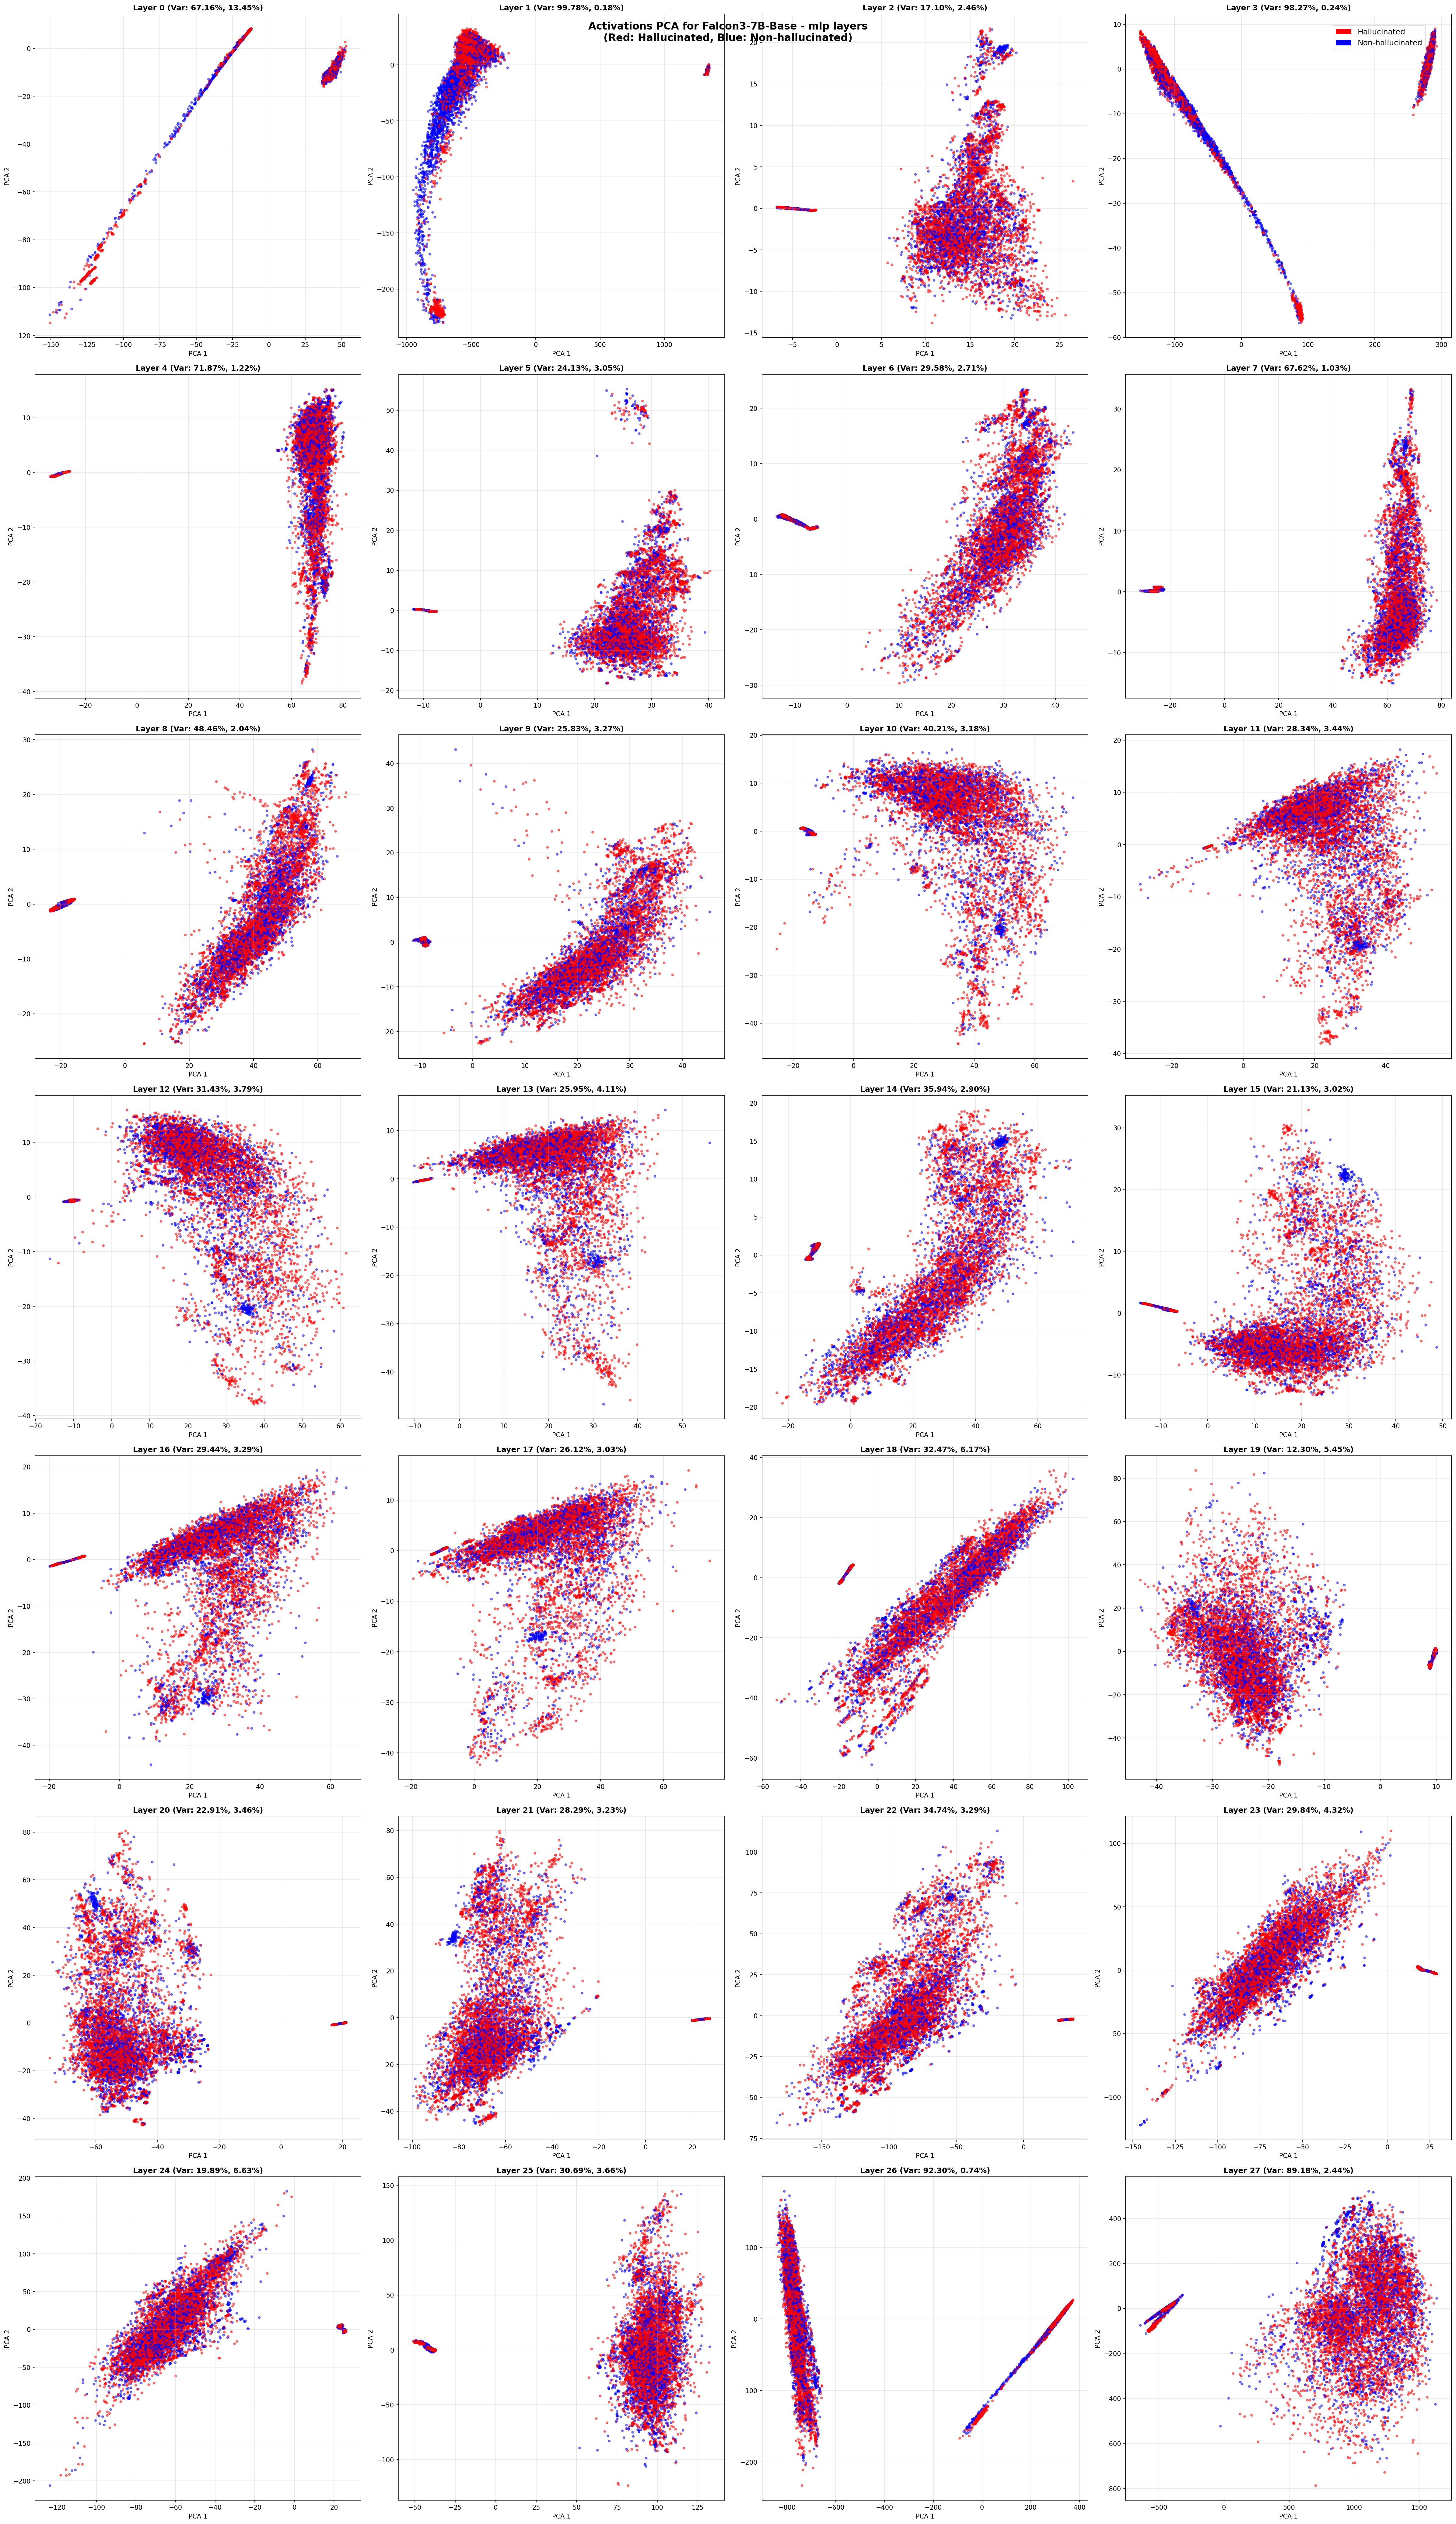
\includegraphics[width=0.9\textwidth]{images/plots/Falcon3-7B-Base_belief_bank_mlp_activations_PCA.png}
    \caption{PCA 2D - Falcon3-7B-Base - MLP Layers}
    \label{fig:pca_falcon_mlp}
\end{figure}

\begin{figure}[h]
    \centering
    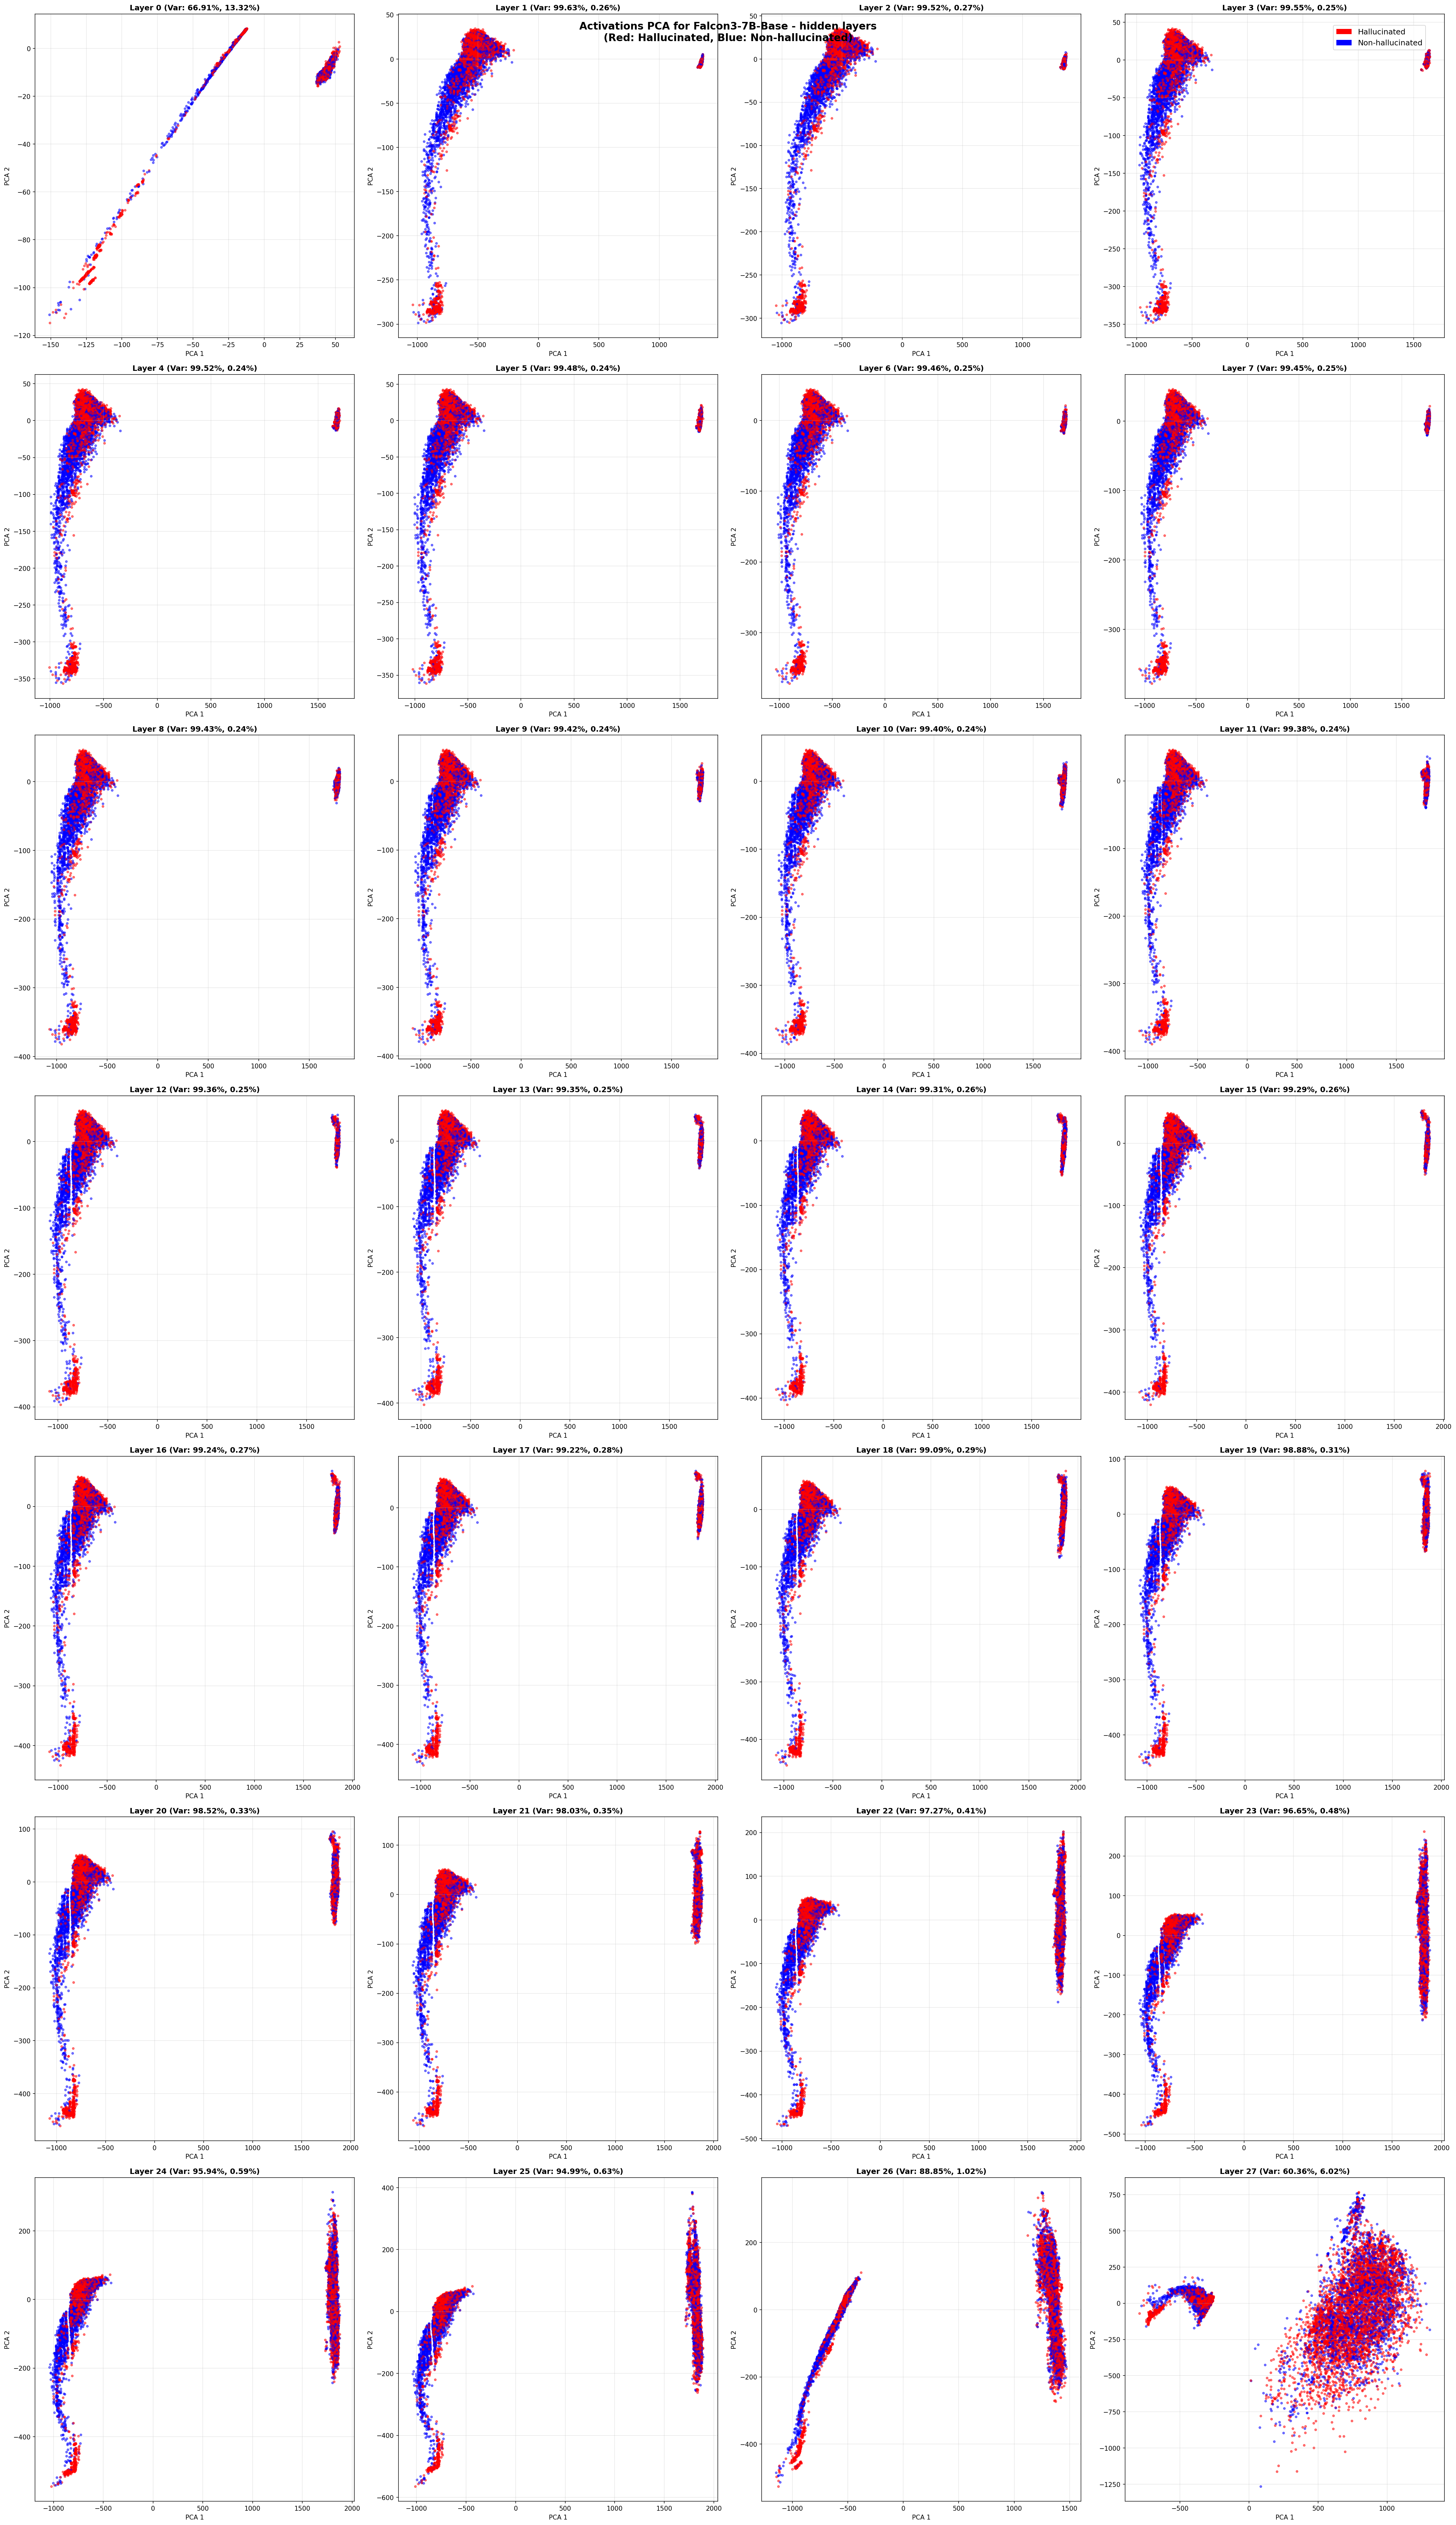
\includegraphics[width=0.9\textwidth]{images/plots/Falcon3-7B-Base_belief_bank_hidden_activations_PCA.png}
    \caption{PCA 2D - Falcon3-7B-Base - Hidden Layers}
    \label{fig:pca_falcon_hidden}
\end{figure}

%\chapter{Model Alignment}
In this appendix, the results of the alignment phase for the various approaches are shown.

\section{Linear Approach}

\begin{figure}[H]
    \centering
    \includegraphics[width=\textwidth, height=0.9\textheight, keepaspectratio]{images/align_plot/alignment_all_layers_Llama-3.1-8B-Instruct_gemma-2-9b-it_belief_bank_constraints.pdf}
    \caption{Alignment between Llama-3.1-8B-Instruct and Gemma-2-9B-IT for Belief Bank Constraints}
    \label{fig:alignment-llama-gemma-constraints}
\end{figure}

\begin{figure}[H]
    \centering
    \includegraphics[width=\textwidth, height=0.9\textheight, keepaspectratio]{images/align_plot/alignment_all_layers_Llama-3.1-8B-Instruct_gemma-2-9b-it_belief_bank_facts.pdf}
    \caption{Alignment between Llama-3.1-8B-Instruct and Gemma-2-9B-IT for Belief Bank Facts}
    \label{fig:alignment-llama-gemma-facts}
\end{figure}

\begin{figure}[H]
    \centering
    \includegraphics[width=\textwidth, height=0.9\textheight, keepaspectratio]{images/align_plot/alignment_all_layers_Llama-3.1-8B-Instruct_gemma-2-9b-it_halu_eval.pdf}
    \caption{Alignment between Llama-3.1-8B-Instruct and Gemma-2-9B-IT for Halu Eval}
    \label{fig:alignment-llama-gemma-halu}
\end{figure}

\begin{figure}[H]
    \centering
    \includegraphics[width=\textwidth, height=0.9\textheight, keepaspectratio]{images/align_plot/alignment_all_layers_Qwen2.5-7B_Falcon3-7B-Base_belief_bank_facts.pdf}
    \caption{Alignment between Qwen2.5-7B and Falcon3-7B-Base for Belief Bank Facts}
    \label{fig:alignment-qwen-falcon-facts}
\end{figure}

\section{Approach 1}

\begin{figure}[H]
    \centering
    \includegraphics[width=\textwidth, height=0.9\textheight, keepaspectratio]{images/align_plot/alignment_approach1_all_layers_Llama-3.1-8B-Instruct_gemma-2-9b-it_belief_bank_constraints.pdf}
    \caption{Alignment (Approach 1) between Llama-3.1-8B-Instruct and Gemma-2-9B-IT for Belief Bank Constraints}
    \label{fig:alignment-app1-llama-gemma-constraints}
\end{figure}

\begin{figure}[H]
    \centering
    \includegraphics[width=\textwidth, height=0.9\textheight, keepaspectratio]{images/align_plot/alignment_approach1_all_layers_Llama-3.1-8B-Instruct_gemma-2-9b-it_belief_bank_facts.pdf}
    \caption{Alignment (Approach 1) between Llama-3.1-8B-Instruct and Gemma-2-9B-IT for Belief Bank Facts}
    \label{fig:alignment-app1-llama-gemma-facts}
\end{figure}

\begin{figure}[H]
    \centering
    \includegraphics[width=\textwidth, height=0.9\textheight, keepaspectratio]{images/align_plot/alignment_approach1_all_layers_Llama-3.1-8B-Instruct_gemma-2-9b-it_halu_eval.pdf}
    \caption{Alignment (Approach 1) between Llama-3.1-8B-Instruct and Gemma-2-9B-IT for Halu Eval}
    \label{fig:alignment-app1-llama-gemma-halu}
\end{figure}

\begin{figure}[H]
    \centering
    \includegraphics[width=\textwidth, height=0.9\textheight, keepaspectratio]{images/align_plot/alignment_approach1_all_layers_Qwen2.5-7B_Falcon3-7B-Base_belief_bank_facts.pdf}
    \caption{Alignment (Approach 1) between Qwen2.5-7B and Falcon3-7B-Base for Belief Bank Facts}
    \label{fig:alignment-app1-qwen-falcon-facts}
\end{figure}

\section{Hybrid Approach}

\begin{figure}[H]
    \centering
    \includegraphics[width=\textwidth, height=0.9\textheight, keepaspectratio]{images/align_plot/alignment_hybrid_all_layers_Llama-3.1-8B-Instruct_gemma-2-9b-it_belief_bank_constraints.pdf}
    \caption{Hybrid Alignment between Llama-3.1-8B-Instruct and Gemma-2-9B-IT for Belief Bank Constraints}
    \label{fig:alignment-hybrid-llama-gemma-constraints}
\end{figure}

\begin{figure}[H]
    \centering
    \includegraphics[width=\textwidth, height=0.9\textheight, keepaspectratio]{images/align_plot/alignment_hybrid_all_layers_Llama-3.1-8B-Instruct_gemma-2-9b-it_belief_bank_facts.pdf}
    \caption{Hybrid Alignment between Llama-3.1-8B-Instruct and Gemma-2-9B-IT for Belief Bank Facts}
    \label{fig:alignment-hybrid-llama-gemma-facts}
\end{figure}

\begin{figure}[H]
    \centering
    \includegraphics[width=\textwidth, height=0.9\textheight, keepaspectratio]{images/align_plot/alignment_hybrid_all_layers_Llama-3.1-8B-Instruct_gemma-2-9b-it_halu_eval.pdf}
    \caption{Hybrid Alignment between Llama-3.1-8B-Instruct and Gemma-2-9B-IT for Halu Eval}
    \label{fig:alignment-hybrid-llama-gemma-halu}
\end{figure}

\begin{figure}[H]
    \centering
    \includegraphics[width=\textwidth, height=0.9\textheight, keepaspectratio]{images/align_plot/alignment_hybrid_all_layers_Qwen2.5-7B_Falcon3-7B-Base_belief_bank_facts.pdf}
    \caption{Hybrid Alignment between Qwen2.5-7B and Falcon3-7B-Base for Belief Bank Facts}
    \label{fig:alignment-hybrid-qwen-falcon-facts}
\end{figure}

\section{Projected Approach}

\begin{figure}[H]
    \centering
    \includegraphics[width=\textwidth, height=0.9\textheight, keepaspectratio]{images/align_plot/alignment_projected_all_layers_Llama-3.1-8B-Instruct_gemma-2-9b-it_belief_bank_constraints.pdf}
    \caption{Projected Alignment between Llama-3.1-8B-Instruct and Gemma-2-9B-IT for Belief Bank Constraints}
    \label{fig:alignment-proj-llama-gemma-constraints}
\end{figure}

\begin{figure}[H]
    \centering
    \includegraphics[width=\textwidth, height=0.9\textheight, keepaspectratio]{images/align_plot/alignment_projected_all_layers_Llama-3.1-8B-Instruct_gemma-2-9b-it_belief_bank_facts.pdf}
    \caption{Projected Alignment between Llama-3.1-8B-Instruct and Gemma-2-9B-IT for Belief Bank Facts}
    \label{fig:alignment-proj-llama-gemma-facts}
\end{figure}

\begin{figure}[H]
    \centering
    \includegraphics[width=\textwidth, height=0.9\textheight, keepaspectratio]{images/align_plot/alignment_projected_all_layers_Llama-3.1-8B-Instruct_gemma-2-9b-it_halu_eval.pdf}
    \caption{Projected Alignment between Llama-3.1-8B-Instruct and Gemma-2-9B-IT for Halu Eval}
    \label{fig:alignment-proj-llama-gemma-halu}
\end{figure}

\begin{figure}[H]
    \centering
    \includegraphics[width=\textwidth, height=0.9\textheight, keepaspectratio]{images/align_plot/alignment_projected_all_layers_Qwen2.5-7B_Falcon3-7B-Base_belief_bank_facts.pdf}
    \caption{Projected Alignment between Qwen2.5-7B and Falcon3-7B-Base for Belief Bank Facts}
    \label{fig:alignment-proj-qwen-falcon-facts}
\end{figure}




\end{appendices}

\end{document}
